% !Mode:: "TeX:UTF-8"
% !TEX encoding = UTF-8 Unicode

%----------------------------------------------------------------------------------------
% 机器翻译:基础与模型
% Machine Translation: Foundations and Models
%
% Copyright 2020
% 肖桐(xiaotong@mail.neu.edu.cn) 朱靖波 (zhujingbo@mail.neu.edu.cn)
%----------------------------------------------------------------------------------------

%----------------------------------------------------------------------------------------
%    CONFIGURATIONS
%----------------------------------------------------------------------------------------

\renewcommand\figurename{图}%将figure改为图
\renewcommand\tablename{表}%将figure改为图
\chapterimage{fig-NEU-5.jpg} % Chapter heading image

%----------------------------------------------------------------------------------------
%	CHAPTER 17
%----------------------------------------------------------------------------------------

\chapter{多模态、多层次机器翻译}

\parinterval 基于上下文的翻译是机器翻译的一个重要分支。传统方法中,机器翻译通常被定义为对一个句子进行翻译的任务。但是,现实中每句话往往不是独立出现的。比如,人们会使用语音进行表达,或者通过图片来传递信息,这些语音和图片内容都可以伴随着文字一起出现在翻译场景中。此外,句子往往存在于段落或者篇章之中,如果要理解这个句子,也需要整个段落或者篇章的信息,而这些上下文信息都是机器翻译可以利用的。

\parinterval 本章在句子级翻译的基础上将问题扩展为更大的上下文中的翻译,具体包括语音翻译、图像翻译、篇章翻译三个主题。这些问题均为机器翻译应用中的真实需求。同时,使用多模态等信息也是当下自然语言处理的热点研究方向之一。

%----------------------------------------------------------------------------------------
%    NEW SECTION
%----------------------------------------------------------------------------------------

\section{机器翻译需要更多的上下文}

\parinterval 长期以来,机器翻译都是指句子级翻译。主要原因在于,句子级的翻译建模可以大大简化问题,使得机器翻译方法更容易被实践和验证。但是人类使用语言的过程并不是孤立地在一个个句子上进行的。这个问题可以类比于人类学习语言的过程:小孩成长过程中会接受视觉、听觉、触觉等多种信号,这些信号的共同作用使得他们产生对客观世界的“认识”,同时促使他们使用“语言”进行表达。从这个角度说,语言能力并不是由单一因素形成的,它往往伴随着其他信息的相互作用,比如,当人们翻译一句话的时候,会用到看到的画面、听到的语调、甚至前面说过的句子中的信息。

\parinterval 广义上,当前句子以外的信息都可以被看作一种上下文。比如,图\ref{fig:17-1}中,需要把英语句子“A girl jumps off a bank .”翻译为汉语。但是,其中的“bank”有多个含义,因此仅仅使用英语句子本身的信息可能会将其翻译为“银行”,而非正确的译文“河床”。但是,图\ref{fig:17-1}中也提供了这个英语句子所对应的图片,显然图片中直接展示了河床,这时“bank”是没有歧义的。通常也会把这种使用图片和文字一起进行机器翻译的任务称作{\small\bfnew{多模态机器翻译}}\index{多模态机器翻译}(Multi-Modal Machine Translation)\index{Multi-model Machine Translation}。

%----------------------------------------------
\begin{figure}[htp]
    \centering
\begin{tikzpicture}[node distance = 0]
\tikzstyle{every node}=[scale=0.85]
\begin {scope}
\node[draw=white,scale=0.6] (input) at (0,0){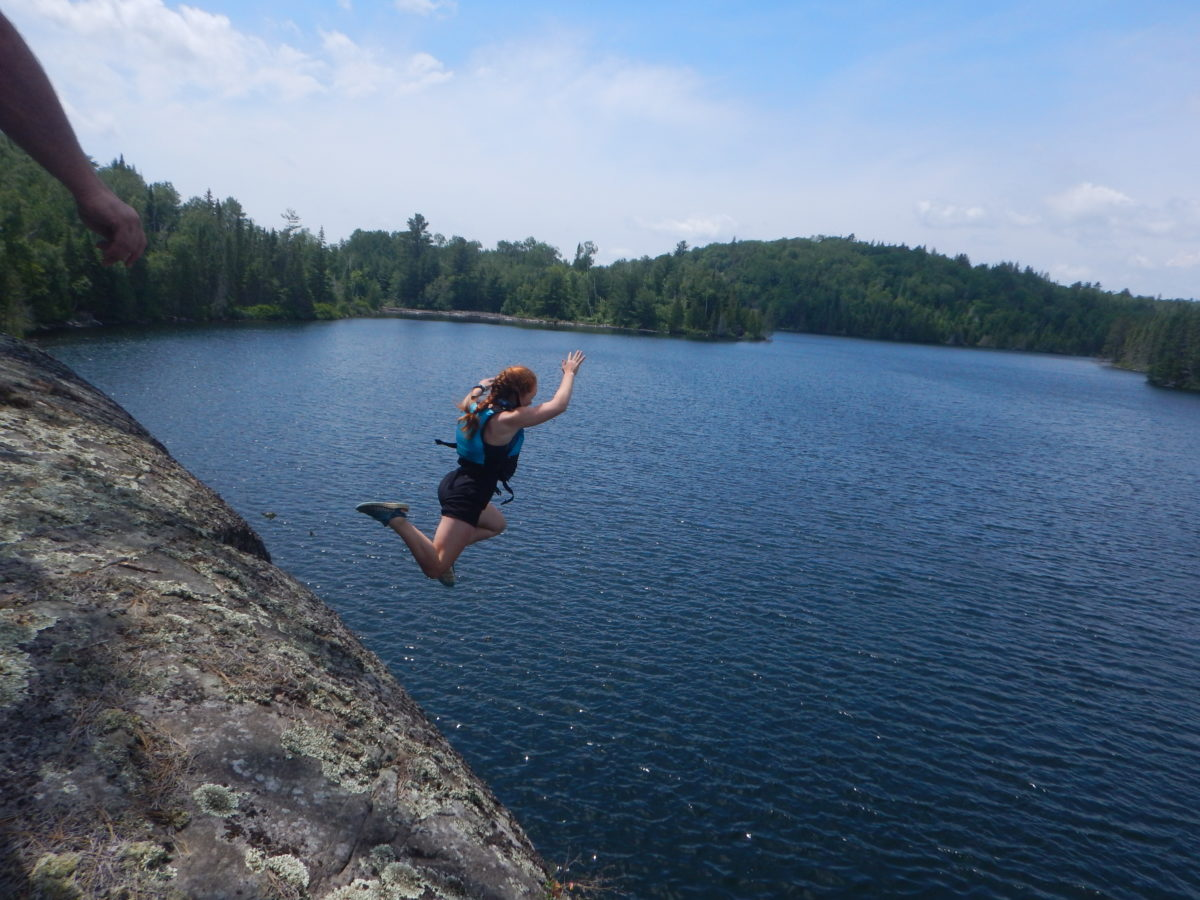
\includegraphics[width=0.62\textwidth]{./Chapter17/Figures/figure-bank-without-attention.jpg}};(1.9,-1.4);
\node[anchor=west] (label1) at ([xshift=-3.5em]input.west) {\begin{tabular}{l}{\normalsize{图片:}}\end{tabular}};
\node[anchor=south] (label2) at ([yshift=-6em]label1.south) {\begin{tabular}{l}{\normalsize{源语言:}}\end{tabular}};
\node[anchor=south] (english1) at ([xshift=-0.28em,yshift=-2.3em]input.south) {\begin{tabular}{l}{\large{A\; girl\; jumps\; off\; a\; {\red{\underline{bank}}}\quad .}}\end{tabular}};

\draw[decorate,decoration={brace,amplitude=4mm},thick] ([xshift=6.3em]input.90) -- ([xshift=0.3em,yshift=-0em]english1.east);

\node[anchor=east,rectangle,thick,rounded corners,minimum width=3.5em,minimum height=2.5em,text centered,draw=black!70,fill=red!25](trans)at ([xshift=7.4em,yshift=5.27em]english1.east){\normalsize{翻译模型}};

\draw[->,thick]([xshift=-1.4em]trans.west) to (trans.west);
\node[anchor=east] (de1) at ([xshift=5.2cm,yshift=-0.1em]trans.east) {\begin{tabular}{l}{\normalsize{目标语言:}}{\normalsize{一个/女孩/从/{\red{河床}}/}}\end{tabular}};
\node[anchor=south] (de2) at ([xshift=1.1em,yshift=-1.5em]de1.south) {\begin{tabular}{l}{\normalsize{上/跳下来/。}} \end{tabular}};
\draw[->,thick](trans.east) to ([xshift=0.5em,yshift=0.1em]de1.west);
\end {scope}
\end{tikzpicture}
    \caption{多模态机器翻译实例}
    \label{fig:17-1}
\end{figure}
%-------------------------------------------
\parinterval {\small\bfnew{模态}}\index{模态}(Modality)\index{Modality}是指某一种信息来源。例如,视觉、听觉、嗅觉、味觉都可以被看作是不同的模态。因此视频、语音、文字等都可以被看作是承载这些模态的媒介。在机器翻译中使用多模态这个概念,是为了区分某些不同于文字的信息。除了图像等视觉模态信息,机器翻译也可以利用听觉模态信息。比如,直接对语音进行翻译,甚至直接用语音表达出翻译结果。

\parinterval 除了不同信息源所引入的上下文,机器翻译也可以利用文字本身的上下文。比如,翻译一篇文章中的某个句子时,可以根据整个篇章的内容进行翻译。显然这种篇章的语境是有助于机器翻译的。在本章接下来的内容中,会对机器翻译中使用不同上下文(多模态和篇章信息)的方法展开讨论。

%----------------------------------------------------------------------------------------
%    NEW SECTION
%----------------------------------------------------------------------------------------
\sectionnewpage
\section{语音翻译}

\parinterval 语音,是人类交流中最常用的一种信息载体。从日常聊天、出国旅游,到国际会议、跨国合作,对于语音翻译的需求不断增加。甚至在有些场景下,用语音进行交互要比用文本进行交互频繁得多。因此,{\small\bfnew{语音翻译}}\index{语音翻译}(Speech Translation)\index{Speech Translation}也成为了语音处理和机器翻译相结合的重要产物。根据目标语言的载体类型,可以将语音翻译分为{\small\bfnew{语音到文本翻译}}\index{语音到文本翻译}(Speech-to-Text Translation)\index{Speech-to-Text Translation}和{\small\bfnew{语音到语音翻译}}\index{语音到语音翻译}(Speech-to-Speech Translation)\index{Speech-to-Speech Translation};基于翻译的实时性,还可以分为{\small\bfnew{实时语音翻译}}\index{实时语音翻译}(即同声传译,Simultaneous Translation)\index{Simultaneous Translation}和{\small\bfnew{离线语音翻译}}(Offline Speech Translation)\index{离线语音翻译}\index{Offline Speech Translation}。本节主要关注离线语音到文本翻译方法(简称为语音翻译),分别从音频处理、级联语音翻译和端到端语音翻译几个角度开展讨论。

%----------------------------------------------------------------------------------------
%    NEW SUB-SECTION
%----------------------------------------------------------------------------------------

\subsection{音频处理}

\parinterval 为了保证对相关内容描述的完整性,这里对语音处理的基本知识作简要介绍。不同于文本,音频本质上是经过若干信号处理之后的{\small\bfnew{波形}}(Waveform)\index{Waveform}。具体来说,声音是一种空气的震动,因此可以被转换为模拟信号。模拟信号是一段连续的信号,经过采样变为离散的数字信号。采样是每隔固定的时间记录一下声音的振幅,采样率表示每秒的采样点数,单位是赫兹(Hz)。采样率越高,采样的结果与原始的语音越相像。通常来说,采样的标准是能够通过离散化的数字信号重现原始语音。日常生活中使用的手机和电脑设备的采样率一般为16kHz,表示每秒16000个采样点;而音频CD的采样率可以达到44.1kHz。 经过进一步的量化,将采样点的值转换为整型数值保存,从而减少占用的存储空间,通常采用的是16位量化。将采样率和量化位数相乘,就可以得到{\small\bfnew{比特率}}\index{比特率}(Bits Per Second,BPS)\index{Bits Per Second},表示音频每秒占用的位数。例如,16kHz采样率和16位量化的音频,比特率为256kb/s。音频处理的整体流程如图\ref{fig:17-2}所示\upcite{洪青阳2020语音识别原理与应用,陈果果2020语音识别实战}。

%----------------------------------------------------------------------------------------------------
\begin{figure}[htp]
\centering
\tikzstyle{process} = [rectangle,very thick,rounded corners,minimum width=4.7cm,minimum height=2.5cm,text centered,draw=black!70,fill=red!20]
\tikzstyle{cir} = [circle,thick,rounded corners,minimum width=0.7cm,text centered,draw=black,fill=green!25]

\begin{tikzpicture}[node distance = 0,scale = 0.7]
\tikzstyle{every node}=[scale=0.7]
\node(voice)[scale=1.0]{声波};
\node(microphone)[rectangle,right of = voice,xshift=1.4cm,yshift=-1cm,minimum width=0.32cm,minimum height=0.35cm,fill=black!85,draw=black!85]{};
\draw[black!85,line width=1.8]([yshift=0.38cm,xshift=-0.4cm]microphone.north)arc(180:360:0.4cm);
\node(microphone_1)[rectangle,minimum width=0.4cm,minimum height=0.8cm,rounded corners=3pt,above of =microphone,yshift=0.75cm,draw=black!85,line width=2.5]{};
\draw[-,black!85,very thick]([yshift=0.4cm,xshift=-0.2cm]microphone.north)--([yshift=0.4cm,xshift=-0cm]microphone.north);
\draw[-,black!85,very thick]([yshift=0.5cm,xshift=-0.2cm]microphone.north)--([yshift=0.5cm,xshift=-0cm]microphone.north);
\draw[-,black!85,very thick]([yshift=0.6cm,xshift=-0.2cm]microphone.north)--([yshift=0.6cm,xshift=-0cm]microphone.north);
\draw[-,black!85,line width=1.8]([yshift=0.6cm,xshift=-0.4cm]microphone.north)--([yshift=0.37cm,xshift=-0.4cm]microphone.north);
\draw[-,black!85,line width=1.8]([yshift=0.6cm,xshift=0.4cm]microphone.north)--([yshift=0.37cm,xshift=0.4cm]microphone.north);
\draw[black!85,line width=1]([yshift=0.8cm,xshift=-0.8cm]microphone.north)arc(-45:45:0.3cm);
\draw[black!85,line width=1]([yshift=0.75cm,xshift=-0.7cm]microphone.north)arc(-45:45:0.4cm);
\draw[black!85,line width=1]([yshift=0.7cm,xshift=-0.6cm]microphone.north)arc(-45:45:0.5cm);

\node(process_1)[process,right of = microphone,xshift=4.7cm,yshift=0.5cm]{};
\node(text_1)[below of = process_1,yshift=-2cm,scale=1.3]{采样};
\draw [very thick,rounded corners=10pt]([xshift=-2.2cm,yshift=-1cm]process_1.center)--([xshift=-1.8cm,yshift=1cm]process_1.center)--([xshift=-1.4cm,yshift=0cm]process_1.center)--([xshift=-1.1cm,yshift=0.8cm]process_1.center)--([xshift=-0.8cm,yshift=-0.4cm]process_1.center)--([xshift=-0.5cm,yshift=0.4cm]process_1.center);
\draw [->,very thick]([xshift=-0.3cm]process_1.center)to([xshift=0.3cm]process_1.center);
\draw [very thick,rounded corners=10pt,densely dotted]([xshift=0.5cm,yshift=-1cm]process_1.center)--([xshift=0.9cm,yshift=1cm]process_1.center)--([xshift=1.3cm,yshift=0cm]process_1.center)--([xshift=1.6cm,yshift=0.8cm]process_1.center)--([xshift=1.9cm,yshift=-0.4cm]process_1.center)--([xshift=2.2cm,yshift=0.4cm]process_1.center);
\node(process_2)[process,fill=blue!20,right of = process_1,xshift=6.6cm]{};
\node(text_2)[below of = process_2,yshift=-2cm,scale=1.3]{量化};
\draw [very thick,rounded corners=10pt,densely dotted]([xshift=-2.2cm,yshift=-1cm]process_2.center)--([xshift=-1.8cm,yshift=1cm]process_2.center)--([xshift=-1.4cm,yshift=0cm]process_2.center)--([xshift=-1.1cm,yshift=0.8cm]process_2.center)--([xshift=-0.8cm,yshift=-0.4cm]process_2.center)--([xshift=-0.5cm,yshift=0.4cm]process_2.center);
\draw [->,very thick]([xshift=-0.3cm]process_2.center)to([xshift=0.3cm]process_2.center);
\draw [very thick,]([xshift=0.5cm,yshift=-0.8cm]process_2.center)--([xshift=0.5cm,yshift=0.3cm]process_2.center)--([xshift=0.7cm,yshift=0.3cm]process_2.center)--([xshift=0.7cm,yshift=0.8cm]process_2.center)--([xshift=1cm,yshift=0.8cm]process_2.center)--([xshift=1cm,yshift=0.2cm]process_2.center)--([xshift=1.3cm,yshift=0.2cm]process_2.center)--([xshift=1.3cm,yshift=0.6cm]process_2.center)--([xshift=1.6cm,yshift=0.6cm]process_2.center)--([xshift=1.6cm,yshift=-0.3cm]process_2.center)--([xshift=1.8cm,yshift=-0.3cm]process_2.center)--([xshift=1.8cm,yshift=0.3cm]process_2.center)--([xshift=2cm,yshift=0.3cm]process_2.center);

\node(text1)[left of = process_1,xshift=-3.2cm,yshift=-0.5cm,align=center]{模拟\\语音信号};
\node(text2)[right of = process_1,xshift=3.3cm,yshift=-0.5cm,align=center]{离散\\时间信号};
\node(text3)[right of = process_2,xshift=3.2cm,yshift=-0.5cm,align=center]{数字离散\\时间信号};

\draw[->,very thick](process_1.east)to(process_2.west);
\draw[->,very thick]([xshift=-1.8cm]process_1.west)to(process_1.west);
\draw[->,very thick](process_2.east)to([xshift=1.8cm]process_2.east);
%%%%音频
\node(signal)[right of = process_2,xshift=5.5cm]{};
\node(text_3)[below of = signal,yshift=-1.98cm,scale=1.3]{语音信号};
\draw[-,thick,]([xshift=-1.2cm]signal.center)--([xshift=1.2cm]signal.center);
\draw[-,thick]([xshift=-1cm,yshift=-0.8cm]signal.center)--([xshift=-0.9cm,yshift=0.4cm]signal.center)--([xshift=-0.8cm,yshift=-0.3cm]signal.center)--([xshift=-0.7cm,yshift=0.7cm]signal.center)--([xshift=-0.6cm,yshift=-0.1cm]signal.center)--([xshift=-0.5cm,yshift=0.3cm]signal.center)--([xshift=-0.4cm,yshift=-0.5cm]signal.center)--([xshift=-0.3cm,yshift=0.7cm]signal.center)--([xshift=-0.2cm,yshift=-0.2cm]signal.center)--([xshift=-0.1cm,yshift=0.4cm]signal.center)--([xshift=0cm,yshift=-0.9cm]signal.center)--([xshift=0.1cm,yshift=0.5cm]signal.center)--([xshift=0.2cm,yshift=-0.4cm]signal.center)--([xshift=0.3cm,yshift=0.3cm]signal.center)--([xshift=0.4cm,yshift=-0.2cm]signal.center)--([xshift=0.5cm,yshift=0.1cm]signal.center)--([xshift=0.6cm,yshift=-0.8cm]signal.center)--([xshift=0.7cm,yshift=0.4cm]signal.center)--([xshift=0.8cm,yshift=-0.6cm]signal.center)--([xshift=0.9cm,yshift=0.7cm]signal.center)--([xshift=1cm,yshift=-0.2cm]signal.center);
\end{tikzpicture}
\caption{音频处理过程}
\label{fig:17-2}
\end{figure}
%----------------------------------------------------------------------------------------------------

\parinterval 经过上面的描述可以看出,音频的表示实际上是一个非常长的采样点序列,这导致了直接使用现有的深度学习技术处理音频序列较为困难。并且,原始的音频信号中可能包含着较多的噪声、环境声或冗余信息,也会对模型产生干扰。因此,一般会对音频序列进行处理来提取声学特征,具体为将长序列的采样点序列转换为短序列的特征向量序列,再用于下游系统。虽然已有一些工作不依赖特征提取,直接在原始的采样点序列上进行声学建模和模型训练\upcite{DBLP:conf/interspeech/SainathWSWV15},但目前的主流方法仍然是基于声学特征进行建模\upcite{DBLP:conf/icassp/MohamedHP12}。

\parinterval 声学特征提取的第一步是预处理。其流程主要是对音频进行{\small\bfnew{预加重}}(Pre-emphasis)\index{预加重}\index{Pre-emphasis}、{\small\bfnew{分帧}}\index{分帧}(Framing)\index{Framing}和{\small\bfnew{加窗}}\index{加窗}(Windowing)\index{Windowing}。预加重是通过增强音频信号中的高频部分来减弱语音中对高频信号的抑制,使频谱更加顺滑。分帧(原理如图\ref{fig:17-3}所示)是基于短时平稳假设,即根据生物学特征,语音信号是一个缓慢变化的过程,10ms$\thicksim$30ms的信号片段是相对平稳的。基于这个假设,一般将每25ms作为一帧来提取特征,这个时间称为{\small\bfnew{帧长}}\index{帧长}(Frame Length)\index{Frame Length}。同时,为了保证不同帧之间的信号平滑性,使每两个相邻帧之间存在一定的重合部分。一般每隔10ms取一帧,这个时长称为{\small\bfnew{帧移}}\index{帧移}(Frame Shift)\index{Frame Shift}。为了缓解分帧带来的频谱泄漏问题,需要对每帧的信号进行加窗处理使其幅度在两段渐变到0,一般采用的是{\small\bfnew{汉明窗}}\index{汉明窗}(Hamming)\index{Hamming}\upcite{洪青阳2020语音识别原理与应用}。
%----------------------------------------------------------------------------------------------------
\begin{figure}[htp]
\centering
\tikzstyle{process} = [rectangle,very thick,rounded corners,minimum width=5cm,minimum height=2.5cm,text centered,draw=black!70,fill=red!25]
\tikzstyle{cir} = [circle,thick,rounded corners,minimum width=0.7cm,text centered,draw=black,fill=green!25]

\begin{tikzpicture}[node distance = 0,scale = 1]
\tikzstyle{every node}=[scale=1]
\node [anchor=center](ori) at (-0.2,-0.2) {0};
\draw[->,thick](-0.5,0)--(5,0)node[below,scale=0.8]{时间};
\draw[->,thick](0,-2)--(0,2)node[left,scale=0.8]{量化值};
\draw[-,thick](0,0)sin(0.7,1.5)cos(1.4,0)sin(2.1,-1.5)cos(2.8,0)sin(3.5,1.5)cos(4.2,0);
\draw[-,thick,dashed](0.5,-1.8)--(0.5,1.8);
\draw[-](1.2,-1.8)--(1.2,1.8);
\draw[-,thick,dashed](1.9,-1.8)--(1.9,1.8);
\draw[<->,thick](0,-1.1)--(1.2,-1.1)node[left,xshift=-0.05cm,yshift=0.15cm,scale=0.6]{帧长};
\draw[<->,thick](0,-1.4)--(0.5,-1.4)node[left,xshift=0.05cm,yshift=-0.25cm,scale=0.6]{帧移};
%\draw[<->,thick](0.5,-1.4)--(1.9,-1.4);
\end{tikzpicture}
\caption{分帧原理图}
\label{fig:17-3}
\end{figure}
%----------------------------------------------------------------------------------------------------

\parinterval 经过了上述的预处理操作,可以得到音频对应的帧序列,之后通过不同的操作来提取不同类型的声学特征。在语音翻译中,比较常用的声学特征为{\small\bfnew{滤波器组}}\index{滤波器组}(Filter-bank,Fbank)\index{Filter-bank}和{\small\bfnew{Mel频率倒谱系数}}\index{Mel频率倒谱系数}(Mel-frequency Cepstral Coefficient,MFCC)\upcite{洪青阳2020语音识别原理与应用}。实际上,提取到的声学特征可以类比于计算机视觉中的像素特征,或者自然语言处理中的词嵌入表示。不同之处在于,声学特征更加复杂多变,可能存在着较多的噪声和冗余信息。此外,相比对应的文字序列,音频提取到的特征序列长度要大十倍以上。比如,人类正常交流中每秒钟一般可以说2-3个字,而每秒钟的语音可以提取得到100帧的特征序列。巨大的长度比差异也为声学特征建模带来了挑战。

%----------------------------------------------------------------------------------------
%    NEW SUB-SECTION
%----------------------------------------------------------------------------------------

\subsection{级联式语音翻译}
\label{sec:cascaded-speech-translation}

\parinterval 实现语音翻译最简单的思路是基于级联的方式,即:先通过{\small\bfnew{自动语音识别}}\index{自动语音识别}(Automatic Speech Recognition,ASR)\index{Automatic Speech Recognition}系统将语音转化为源语言文本,然后利用机器翻译系统将源语言文本翻译为目标语言文本。这种做法的好处在于语音识别和机器翻译模型可以分别进行训练,有很多数据资源以及成熟技术可以分别运用到两个系统中。因此,级联语音翻译是很长时间以来的主流方法,深受工业界的青睐。级联语音翻译主要的流程如图\ref{fig:17-4}所示。

%----------------------------------------------------------------------------------------------------
\begin{figure}[htp]
\centering
\tikzstyle{process} = [rectangle,very thick,rounded corners,minimum width=3.2cm,minimum height=3cm,text centered,draw=black!70,fill=red!20]
\tikzstyle{cir} = [circle,thick,rounded corners,minimum width=0.7cm,text centered,draw=black,fill=green!25]

\begin{tikzpicture}[node distance = 0,scale = 0.5]
\tikzstyle{every node}=[scale=0.5]
\node(process_1)[process]{};
\draw[-,thick]([xshift=-1.2cm]process_1.center)--([xshift=1.2cm]process_1.center);
\draw[-,thick]([xshift=-1cm,yshift=-0.8cm]process_1.center)--([xshift=-0.9cm,yshift=0.4cm]process_1.center)--([xshift=-0.8cm,yshift=-0.3cm]process_1.center)--([xshift=-0.7cm,yshift=0.7cm]process_1.center)--([xshift=-0.6cm,yshift=-0.1cm]process_1.center)--([xshift=-0.5cm,yshift=0.3cm]process_1.center)--([xshift=-0.4cm,yshift=-0.5cm]process_1.center)--([xshift=-0.3cm,yshift=0.7cm]process_1.center)--([xshift=-0.2cm,yshift=-0.2cm]process_1.center)--([xshift=-0.1cm,yshift=0.4cm]process_1.center)--([xshift=0cm,yshift=-0.9cm]process_1.center)--([xshift=0.1cm,yshift=0.5cm]process_1.center)--([xshift=0.2cm,yshift=-0.4cm]process_1.center)--([xshift=0.3cm,yshift=0.3cm]process_1.center)--([xshift=0.4cm,yshift=-0.2cm]process_1.center)--([xshift=0.5cm,yshift=0.1cm]process_1.center)--([xshift=0.6cm,yshift=-0.8cm]process_1.center)--([xshift=0.7cm,yshift=0.4cm]process_1.center)--([xshift=0.8cm,yshift=-0.6cm]process_1.center)--([xshift=0.9cm,yshift=0.7cm]process_1.center)--([xshift=1cm,yshift=-0.2cm]process_1.center);
\node(text_1)[below of = process_1,yshift=-2cm,scale=1.5]{语音信号};
\node(process_2)[process,fill=blue!20,right of = process_1,xshift=7.0cm,text width=4cm,align=center]{\baselineskip=4pt\LARGE{[[0.2,...,0.3], \qquad ..., \qquad  0.3,...,0.5]]}\par};
\node(text_2)[below of = process_2,yshift=-2cm,scale=1.5]{语音特征};
\node(process_3)[process,fill=orange!20,minimum width=6cm,minimum height=5cm,right of = process_2,xshift=8.2cm,text width=4cm,align=center]{};
\node(text_3)[below of = process_3,yshift=-3cm,scale=1.5]{源语言文本及其词格};
\node(cir_s)[cir,very thick, below of = process_3,xshift=-2.2cm,yshift=1.1cm]{\LARGE S};
\node(cir_a)[cir,right of = cir_s,xshift=1cm,yshift=0.8cm]{\LARGE a};
\node(cir_c)[cir,right of = cir_a,xshift=1.2cm,yshift=0cm]{\LARGE c};
\node(cir_f)[cir,right of = cir_c,xshift=1.2cm,yshift=0cm]{\LARGE f};
\node(cir_E)[cir,very thick,right of = cir_f,xshift=1cm,yshift=-0.8cm]{\LARGE E};
\node(cir_b)[cir,right of = cir_s,xshift=1cm,yshift=-0.8cm]{\Large b};
\node(cir_d)[cir,right of = cir_b,xshift=1cm,yshift=0.6cm]{\Large d};
\node(cir_e)[cir, right of = cir_b,xshift=1cm,yshift=-0.8cm]{\LARGE e};
\node(cir_g)[cir,right of = cir_e,xshift=1cm,yshift=0.8cm]{\LARGE g};
\draw[-latex](cir_s)node[above,xshift=0.3cm,yshift=0.4cm]{0.4}to(cir_a);
\draw[-latex](cir_a)node[above,xshift=0.6cm,yshift=0cm]{1}to(cir_c);
\draw[-latex](cir_c)node[above,xshift=0.6cm,yshift=0cm]{1}to(cir_f);
\draw[-latex](cir_f)node[above,xshift=0.6cm,yshift=-0.3cm]{1}to(cir_E);
\draw[-latex](cir_s)node[above,xshift=0.7cm,yshift=-0.4cm]{0.6}to(cir_b);
\draw[-latex](cir_b)node[above,xshift=0.3cm,yshift=0.3cm]{0.8}to(cir_d);
\draw[-latex](cir_b)node[above,xshift=0.7cm,yshift=-0.4cm]{0.2}to(cir_e);
\draw[-latex](cir_e)node[above,xshift=0.3cm,yshift=0.3cm]{1}to(cir_g);
\draw[-latex](cir_d)node[above,xshift=0.7cm,yshift=0cm]{1}to(cir_f);
\draw[-latex](cir_g)node[above,xshift=0.6cm,yshift=0.3cm]{1}--(cir_E);


\node(text)[below of = process_3,yshift=-1.8cm,scale=1.8]{你是谁};
\node(process_4)[process,fill=ugreen!20,right of = process_3,xshift=8.2cm,text width=4cm,align=center]{\Large\textbf{Who are you?}};
\node(text_4)[below of = process_4,yshift=-2cm,scale=1.5]{翻译结果};

\draw[->,very thick](process_1.east)to(process_2.west);
\draw[->,very thick](process_2.east)to(process_3.west);
\draw[->,very thick](process_3.east)to(process_4.west);
\node(arrow_text1)[right of = process_1,xshift=3.2cm,yshift=0.7cm,scale=1.4,align=center]{音频\\特征提取};
\node(arrow_text2)[right of = process_2,xshift=3.6cm,yshift=0.7cm,scale=1.4,align=center]{语音\\识别系统};
\node(arrow_text3)[right of = process_3,xshift=4.5cm,yshift=0.4cm,scale=1.4]{翻译系统};
\end{tikzpicture}
\caption{级联式语音翻译流程示例}
\label{fig:17-4}
\end{figure}
%----------------------------------------------------------------------------------------------------

\parinterval 由于声学特征提取在上一节中已经进行了描述,而且文本翻译可以直接使用本书介绍的统计机器翻译或者神经机器翻译方法。因此下面简要介绍一下语音识别模型,以便读者对级联式语音翻译系统有一个完整的认识。其中的部分概念在后续介绍的端到端语言翻译中也会有所涉及。

\parinterval 传统的语音识别模型和统计机器翻译相似,需要利用声学模型、语言模型和发音词典联合进行识别,系统较为复杂\upcite{DBLP:journals/ftsig/GalesY07,DBLP:journals/taslp/MohamedDH12,DBLP:journals/spm/X12a}。而近些年来,随着神经网络的发展,基于神经网络的端到端语音识别模型逐渐受到关注,训练流程也大大被简化\upcite{DBLP:conf/nips/ChorowskiBSCB15,DBLP:conf/icassp/ChanJLV16}。目前的端到端语音识别模型主要基于序列到序列结构,编码器根据输入的声学特征进一步提取高级特征,解码器根据编码器提取的特征识别对应的文本。在后文中即将介绍的端到端语音翻译模型也是基于十分相似的结构。因此,从某种意义上说,语音识别和翻译所使用的端到端方法与神经机器翻译是一致的。
%----------------------------------------------------------------------------------------------------
\begin{figure}[htp]
\centering
\begin{tikzpicture}
	\tikzstyle{layer}=[draw,rounded corners=2pt,font=\scriptsize,align=center,minimum width=7.1em]
	\tikzstyle{word}=[font=\scriptsize]
%%%%encoder
\node[layer,fill=red!20] (en_sa) at (0,0){Multi-Head \\ Attention};
\node[anchor=south,layer,fill=yellow!20](en_add1) at ([yshift=1.0em]en_sa.north) {Add \& LayerNorm};
\node[layer,anchor=south,fill=green!20] (en_ffn) at ([yshift=1.0em]en_add1.north){Feed Forward \\ Network};
\node[anchor=south,layer,fill=yellow!20](en_add2) at ([yshift=1.0em]en_ffn.north) {Add \& LayerNorm};
\node[draw,circle,inner sep=0pt, minimum size=1em,anchor=north,thick] (en_add) at ([yshift=-1.4em]en_sa.south){};
\draw[thick] (en_add.90) -- (en_add.-90);
\draw[thick] (en_add.0) -- (en_add.180);
\node[layer,anchor=north,fill=yellow!20] (en_cnn) at ([yshift=-1.0em]en_add.south){CNN};
\node[anchor=east,font=\scriptsize,align=center] (en_pos) at ([xshift=-2em]en_add.west){位置编码};
\node[anchor=north,font=\scriptsize,align=center] (en_input) at ([yshift=-1em]en_cnn.south){语音特征\\(FBank/MFCC)};

\draw[->,thick] (en_input.90) -- ([yshift=-0.1em]en_cnn.-90);
\draw[->,thick] ([yshift=0.1em]en_cnn.90) -- ([yshift=-0.1em]en_add.-90);
\draw[->,thick] ([yshift=0.1em]en_add.90) -- ([yshift=-0.1em]en_sa.-90);
\draw[->,thick] ([yshift=0.1em]en_sa.90) -- ([yshift=-0.1em]en_add1.-90);
\draw[->,thick] ([yshift=0.1em]en_add1.90) -- ([yshift=-0.1em]en_ffn.-90);
\draw[->,thick] ([yshift=0.1em]en_ffn.90) --([yshift=-0.1em]en_add2.-90);
\draw[->,rounded corners=2pt,thick] ([yshift=-0.6em]en_sa.south)--([yshift=-0.6em,xshift=-4.0em]en_sa.south)--([xshift=-0.43em]en_add1.west)--(en_add1.west);
\draw[->,rounded corners=2pt,thick] ([yshift=-0.6em]en_ffn.south)--([yshift=-0.6em,xshift=-4.0em]en_ffn.south)--([xshift=-0.43em]en_add2.west)--(en_add2.west);

%%%%decoder
\node[draw,circle,inner sep=0pt, minimum size=1em,anchor=west,thick] (de_add) at ([xshift=9em]en_add.east){};
\draw[thick] (de_add.90) -- (de_add.-90);
\draw[thick] (de_add.0) -- (de_add.180);
\node[layer,anchor=south,fill=red!20] (de_sa) at ([yshift=1.4em]de_add.north){Masked \\Multi-Head\\Attention};
\node[anchor=south,layer,fill=yellow!20](de_add1) at ([yshift=1.0em]de_sa.north) {Add \& LayerNorm};
\node[layer,anchor=south,fill=red!20] (de_ca) at ([yshift=1.0em]de_add1.north){Multi-Head \\ Attention};
\node[anchor=south,layer,fill=yellow!20](de_add2) at ([yshift=1.0em]de_ca.north) {Add \& LayerNorm};
\node[layer,anchor=south,fill=green!20] (de_ffn) at ([yshift=1.0em]de_add2.north){Feed Forward \\ Network};
\node[anchor=south,layer,fill=yellow!20](de_add3) at ([yshift=1.0em]de_ffn.north) {Add \& LayerNorm};
\node[layer,anchor=south,fill=blue!20] (sf) at ([yshift=1.2em]de_add3.north){Softmax};
\node[anchor=north,font=\scriptsize,align=center] (de_input) at ([yshift=-1.1em]de_add.south){标注文本\\编码表示};

\node[anchor=west,font=\scriptsize,align=center] (de_pos) at ([xshift=2em]de_add.east){位置编码};

\draw[->,thick] (de_input.90) -- ([yshift=-0.1em]de_add.-90);
\draw[->,thick] ([yshift=0.1em]de_add.90) -- ([yshift=-0.1em]de_sa.-90);
\draw[->,thick] ([yshift=0.1em]de_sa.90) -- ([yshift=-0.1em]de_add1.-90);
\draw[->,thick] ([yshift=0.1em]de_add1.90) -- ([yshift=-0.1em]de_ca.-90);
\draw[->,thick] ([yshift=0.1em]de_ca.90) -- ([yshift=-0.1em]de_add2.-90);
\draw[->,thick] ([yshift=0.1em]de_add2.90) -- ([yshift=-0.1em]de_ffn.-90);
\draw[->,thick] ([yshift=0.1em]de_ffn.90) -- ([yshift=-0.1em]de_add3.-90);
\draw[->,thick] ([yshift=0.1em]de_add3.90) -- ([yshift=-0.1em]sf.-90);
\draw[->,thick] ([yshift=0.1em]sf.90) -- ([yshift=1.0em]sf.90);
\draw[->,thick] ([xshift=0.1em]en_pos.0) -- ([xshift=-0.1em]en_add.180);
\draw[->,thick] ([xshift=-0.1em]de_pos.180) -- ([xshift=0.1em]de_add.0);
\draw[->,rounded corners=2pt,thick] ([yshift=-0.6em]de_sa.south)--([yshift=-0.6em,xshift=4.0em]de_sa.south)--([xshift=0.43em]de_add1.east)--(de_add1.east);
\draw[->,rounded corners=2pt,thick] ([yshift=-0.6em]de_ca.south)--([yshift=-0.6em,xshift=4.0em]de_ca.south)--([xshift=0.43em]de_add2.east)--(de_add2.east);
\draw[->,rounded corners=2pt,thick] ([yshift=-0.6em]de_ffn.south)--([yshift=-0.6em,xshift=4.0em]de_ffn.south)--([xshift=0.43em]de_add3.east)--(de_add3.east);

\draw[->,rounded corners=2pt,thick] ([yshift=0.1em]en_add2.90) -- ([yshift=1.5em]en_add2.90) -- ([xshift=5.0em,yshift=1.5em]en_add2.90) -- ([xshift=-1.5em]de_ca.west) -- ([xshift=-0.1em]de_ca.west);


\begin{pgfonlayer}{background}
\node[draw=ugreen,rounded corners=2pt,inner xsep=6pt,inner ysep=8pt,dashed,thick,xshift=-0.2em,yshift=-0.2em][fit=(en_add1)(en_add2)(en_sa)(en_ffn)](box1){};
\node[draw=red,rounded corners=2pt,inner xsep=6pt,inner ysep=8pt,dashed,thick,xshift=0.2em,yshift=-0.2em][fit=(de_sa)(de_ca)(de_ffn)(de_add3)](box2){};
\end{pgfonlayer}

\node[anchor=east,font=\scriptsize,text=ugreen] at ([xshift=-0.1em]box1.west){$N \times$};
\node[anchor=west,font=\scriptsize,text=red] at ([xshift=0.1em]box2.east){$\times N$};
\node[anchor=east,font=\scriptsize] at ([xshift=-0.1em]en_cnn.west){$2 \times$};
\node[anchor=east,font=\scriptsize,align=center,text=ugreen] at ([xshift=-0.1em,yshift=3em]box1.west){ASR \\ 编码器};
\node[anchor=west,font=\scriptsize,align=center,text=red] at ([xshift=0.1em,yshift=5em]box2.east){ASR \\ 解码器};
\end{tikzpicture}
\setlength{\abovecaptionskip}{-0.2em}
\caption{基于Transformer的语音识别模型}
\label{fig:17-5}
\end{figure}
%----------------------------------------------------------------------------------------------------

\vspace{-1em}
\parinterval 语音识别目前广泛使用基于Transformer的模型结构(见{\chaptertwelve}),如图\ref{fig:17-5}所示。可以看出,相比文本翻译,模型结构上唯一的区别在于编码器的输入为声学特征,以及编码器底层会使用额外的卷积层来减小输入序列的长度。这是由于语音对应的特征序列过长,在计算注意力模型的时候,会占用大量的内存/显存,并增加训练时间。因此,一个常用的做法是在语音特征上进行两层步长为2的卷积操作,从而将输入序列的长度缩小为之前的1/4。通过使用大量的语音-标注平行数据对模型进行训练,可以得到高质量的语音识别模型。

\parinterval 为了降低语音识别的错误对下游系统的影响,通常也会用词格来取代One-best语音识别结果。另一种思路是通过一个后处理模型修正识别结果中的错误,再送给文本翻译模型进行翻译。也可以进一步对文本做{\small\bfnew{顺滑}}\index{顺滑}(Disfluency Detection\index{Disfluency Detection})处理,使得送给翻译系统的文本更加干净、流畅,比如除去一些导致停顿的语气词。这一做法在工业界得到了广泛应用,但由于每个模型只能串行地计算,也会带来额外的计算代价以及运算时间。另外一种思路是训练更加健壮的文本翻译模型,使其可以处理输入中存在的噪声或误差\upcite{DBLP:conf/acl/LiuTMCZ18}。

%----------------------------------------------------------------------------------------
%    NEW SUB-SECTION
%----------------------------------------------------------------------------------------

\subsection{端到端语音翻译}

\parinterval 级联语音翻译模型结构简单、易于实现,但不可避免地存在一些缺陷:

%----------------------------------------------------------------------------------------------------
\begin{itemize}
    \item {\small\bfnew{错误传播问题}}。级联模型导致的一个很严重的问题在于,语音识别模型得到的文本如果存在错误,这些错误很可能在翻译过程中被放大,从而使最后翻译结果出现比较大的偏差。比如识别时在句尾少生成了个“吗”,会导致翻译模型将疑问句翻译为陈述句。
    \vspace{0.5em}
    \item {\small\bfnew{翻译效率问题}}。由于语音识别模型和文本标注模型只能串行地计算,翻译效率相对较低,而实际很多场景中都需要实现低延时的翻译。
    \vspace{0.5em}
    \item {\small\bfnew{语音中的副语言信息丢失}}。将语音识别为文本的过程中,语音中包含的语气、情感、音调等信息会丢失,而同一句话在不同的语气中表达的意思很可能是不同的。尤其是在实际应用中,由于语音识别结果通常并不包含标点,还需要额外的后处理模型将标点还原,也会带来额外的计算代价。
\end{itemize}
%----------------------------------------------------------------------------------------------------

%----------------------------------------------------------------------------------------------------
\begin{figure}[htp]
\centering
\begin{tikzpicture}
	\tikzstyle{layer}=[draw,rounded corners=2pt,font=\scriptsize,align=center,minimum width=7.1em]
	\tikzstyle{word}=[font=\scriptsize]
%%%%encoder
\node[layer,fill=red!20] (en_sa) at (0,0){Multi-Head \\ Attention};
\node[anchor=south,layer,fill=yellow!20](en_add1) at ([yshift=1.0em]en_sa.north) {Add \& LayerNorm};
\node[layer,anchor=south,fill=green!20] (en_ffn) at ([yshift=1.0em]en_add1.north){Feed Forward \\ Network};
\node[anchor=south,layer,fill=yellow!20](en_add2) at ([yshift=1.0em]en_ffn.north) {Add \& LayerNorm};
\node[draw,circle,inner sep=0pt, minimum size=1em,anchor=north,thick] (en_add) at ([yshift=-1.4em]en_sa.south){};
\draw[thick] (en_add.90) -- (en_add.-90);
\draw[thick] (en_add.0) -- (en_add.180);
\node[layer,anchor=north,fill=yellow!20] (en_cnn) at ([yshift=-1.0em]en_add.south){CNN};
\node[anchor=east,font=\scriptsize,align=center] (en_pos) at ([xshift=-2em]en_add.west){位置编码};
\node[anchor=north,font=\scriptsize,align=center] (en_input) at ([yshift=-1em]en_cnn.south){源语言语音特征\\(FBank/MFCC)};

\draw[->,thick] (en_input.90) -- ([yshift=-0.1em]en_cnn.-90);
\draw[->,thick] ([yshift=0.1em]en_cnn.90) -- ([yshift=-0.1em]en_add.-90);
\draw[->,thick] ([yshift=0.1em]en_add.90) -- ([yshift=-0.1em]en_sa.-90);
\draw[->,thick] ([yshift=0.1em]en_sa.90) -- ([yshift=-0.1em]en_add1.-90);
\draw[->,thick] ([yshift=0.1em]en_add1.90) -- ([yshift=-0.1em]en_ffn.-90);
\draw[->,thick] ([yshift=0.1em]en_ffn.90) --([yshift=-0.1em]en_add2.-90);
\draw[->,rounded corners=2pt,thick] ([yshift=-0.6em]en_sa.south)--([yshift=-0.6em,xshift=-4.0em]en_sa.south)--([xshift=-0.43em]en_add1.west)--(en_add1.west);
\draw[->,rounded corners=2pt,thick] ([yshift=-0.6em]en_ffn.south)--([yshift=-0.6em,xshift=-4.0em]en_ffn.south)--([xshift=-0.43em]en_add2.west)--(en_add2.west);

%%%%decoder
\node[draw,circle,inner sep=0pt, minimum size=1em,anchor=west,thick] (de_add) at ([xshift=9em]en_add.east){};
\draw[thick] (de_add.90) -- (de_add.-90);
\draw[thick] (de_add.0) -- (de_add.180);
\node[layer,anchor=south,fill=red!20] (de_sa) at ([yshift=1.4em]de_add.north){Masked \\Multi-Head\\Attention};
\node[anchor=south,layer,fill=yellow!20](de_add1) at ([yshift=1.0em]de_sa.north) {Add \& LayerNorm};
\node[layer,anchor=south,fill=red!20] (de_ca) at ([yshift=1.0em]de_add1.north){Multi-Head \\ Attention};
\node[anchor=south,layer,fill=yellow!20](de_add2) at ([yshift=1.0em]de_ca.north) {Add \& LayerNorm};
\node[layer,anchor=south,fill=green!20] (de_ffn) at ([yshift=1.0em]de_add2.north){Feed Forward \\ Network};
\node[anchor=south,layer,fill=yellow!20](de_add3) at ([yshift=1.0em]de_ffn.north) {Add \& LayerNorm};
\node[layer,anchor=south,fill=blue!20] (sf) at ([yshift=1.2em]de_add3.north){Softmax};
\node[anchor=north,font=\scriptsize,align=center] (de_input) at ([yshift=-1.1em]de_add.south){目标语言文本\\编码表示};

\node[anchor=west,font=\scriptsize,align=center] (de_pos) at ([xshift=2em]de_add.east){位置编码};

\draw[->,thick] (de_input.90) -- ([yshift=-0.1em]de_add.-90);
\draw[->,thick] ([yshift=0.1em]de_add.90) -- ([yshift=-0.1em]de_sa.-90);
\draw[->,thick] ([yshift=0.1em]de_sa.90) -- ([yshift=-0.1em]de_add1.-90);
\draw[->,thick] ([yshift=0.1em]de_add1.90) -- ([yshift=-0.1em]de_ca.-90);
\draw[->,thick] ([yshift=0.1em]de_ca.90) -- ([yshift=-0.1em]de_add2.-90);
\draw[->,thick] ([yshift=0.1em]de_add2.90) -- ([yshift=-0.1em]de_ffn.-90);
\draw[->,thick] ([yshift=0.1em]de_ffn.90) -- ([yshift=-0.1em]de_add3.-90);
\draw[->,thick] ([yshift=0.1em]de_add3.90) -- ([yshift=-0.1em]sf.-90);
\draw[->,thick] ([yshift=0.1em]sf.90) -- ([yshift=1.0em]sf.90);
\draw[->,thick] ([xshift=0.1em]en_pos.0) -- ([xshift=-0.1em]en_add.180);
\draw[->,thick] ([xshift=-0.1em]de_pos.180) -- ([xshift=0.1em]de_add.0);
\draw[->,rounded corners=2pt,thick] ([yshift=-0.6em]de_sa.south)--([yshift=-0.6em,xshift=4.0em]de_sa.south)--([xshift=0.43em]de_add1.east)--(de_add1.east);
\draw[->,rounded corners=2pt,thick] ([yshift=-0.6em]de_ca.south)--([yshift=-0.6em,xshift=4.0em]de_ca.south)--([xshift=0.43em]de_add2.east)--(de_add2.east);
\draw[->,rounded corners=2pt,thick] ([yshift=-0.6em]de_ffn.south)--([yshift=-0.6em,xshift=4.0em]de_ffn.south)--([xshift=0.43em]de_add3.east)--(de_add3.east);

\draw[->,rounded corners=2pt,thick] ([yshift=0.1em]en_add2.90) -- ([yshift=1.5em]en_add2.90) -- ([xshift=5.0em,yshift=1.5em]en_add2.90) -- ([xshift=-1.5em]de_ca.west) -- ([xshift=-0.1em]de_ca.west);


\begin{pgfonlayer}{background}
\node[draw=ugreen,rounded corners=2pt,inner xsep=6pt,inner ysep=8pt,dashed,thick,xshift=-0.2em,yshift=-0.2em][fit=(en_add1)(en_add2)(en_sa)(en_ffn)](box1){};
\node[draw=red,rounded corners=2pt,inner xsep=6pt,inner ysep=8pt,dashed,thick,xshift=0.2em,yshift=-0.2em][fit=(de_sa)(de_ca)(de_ffn)(de_add3)](box2){};
\end{pgfonlayer}

\node[anchor=east,font=\scriptsize,text=ugreen] at ([xshift=-0.1em]box1.west){$N \times$};
\node[anchor=west,font=\scriptsize,text=red] at ([xshift=0.1em]box2.east){$\times N$};
\node[anchor=east,font=\scriptsize] at ([xshift=-0.1em]en_cnn.west){$2 \times$};
\node[anchor=east,font=\scriptsize,align=center,text=ugreen] at ([xshift=-0.1em,yshift=3em]box1.west){ST \\ 编码器};
\node[anchor=west,font=\scriptsize,align=center,text=red] at ([xshift=0.1em,yshift=5em]box2.east){ST \\ 解码器};
\end{tikzpicture}
\setlength{\abovecaptionskip}{-0.2em}
\caption{基于Transformer的端到端语音翻译模型}
\label{fig:17-7}
\end{figure}
%----------------------------------------------------------------------------------------------------

\parinterval 针对级联语音翻译模型存在的缺陷,研究人员提出了{\small\bfnew{端到端的语音翻译模型}}\index{端到端的语音翻译模型}(End-to-End Speech Translation,E2E-ST)\index{End-to-End Speech Translation}\upcite{DBLP:conf/naacl/DuongACBC16,DBLP:conf/interspeech/WeissCJWC17,DBLP:journals/corr/BerardPSB16},也就是模型的输入是源语言语音,输出是对应的目标语言文本。相比级联模型,端到端模型有如下优点:

%----------------------------------------------------------------------------------------------------
\begin{itemize}
    \vspace{0.5em}
    \item 端到端模型不需要多阶段的处理,因此避免了错误传播问题。
    \vspace{0.5em}
    \item 同样地,端到端模型所涉及的模块更少,容易控制模型体积。
    \vspace{0.5em}
    \item 端到端模型语音信号可以直接作用于翻译过程,因此可以使得副语言信息得以体现。
    \vspace{0.5em}
\end{itemize}
%----------------------------------------------------------------------------------------------------

\parinterval 以Transformer模型为例,图\ref{fig:17-7}展示了端到端语音翻译的架构(下文中语音翻译模型均指端到端的模型)。该模型采用的也是序列到序列架构,编码器的输入是从语音中提取的特征(比如FBank特征)。编码器底层采用和语音识别模型相同的卷积结构来降低序列的长度(见\ref{sec:cascaded-speech-translation}节)。之后的流程和标准的神经机器翻译是完全一致的,编码器对语音特征进行编码,解码器根据编码结果生成目标语言的翻译结果。

\parinterval 虽然端到端语音翻译模型解决了级联模型存在的问题,但同时也面临着两个严峻的问题:

%----------------------------------------------------------------------------------------------------
\begin{itemize}
    \vspace{0.5em}
    \item {\small\bfnew{训练数据稀缺}}。虽然语音识别和文本翻译的训练数据都很多,但是直接由源语言语音到目标语言文本的平行数据十分有限,因此端到端语音翻译天然地就是一种低资源翻译任务。
    \vspace{0.5em}
    \item {\small\bfnew{建模复杂度更高}}。在语音识别中,模型是学习如何生成语音对应的文字序列,输入和输出的对齐比较简单,不涉及到调序的问题。在文本翻译中,模型要学习如何生成源语言序列对应的目标语言序列,仅需要学习不同语言之间的映射,不涉及到模态的转换。而语音翻译模型需要学习从语音到目标语言文本的生成,任务更加复杂。
    \vspace{0.5em}
\end{itemize}
%----------------------------------------------------------------------------------------------------

\parinterval 针对这两个问题,研究人员们也提出了很多方法进行缓解,包括多任务学习、迁移学习等,主要思想都是利用语音识别或文本翻译数据来指导模型的学习。并且,文本翻译的很多方法对语音翻译技术的发展提供了思路。如何将其他领域现有的工作在语音翻译任务上验证,也是语音翻译研究人员当前所关注的\upcite{DBLP:conf/mtsummit/GangiNCDT19}。

%----------------------------------------------------------------------------------------
%    NEW SUBSUB-SECTION
%----------------------------------------------------------------------------------------
\subsubsection{1. 多任务学习}

\parinterval 一种思路是进行多任务学习,让模型在训练过程中得到更多的监督信息。使用多个任务强化主任务(机器翻译),在本书的{\chapterfifteen}和{\chaptersixteen}也有所涉及。从这个角度说,机器翻译中很多问题的解决手段都是一致的。

\parinterval 语音翻译中多任务学习主要借助语音对应的标注信息,也就是源语言文本。{\small\bfnew{连接时序分类}}\index{连接时序分类}(Connectionist Temporal Classification,CTC)\index{Connectionist Temporal Classification}\upcite{DBLP:conf/icml/GravesFGS06}是语音处理中最简单有效的一种多任务学习方法\upcite{DBLP:journals/jstsp/WatanabeHKHH17,DBLP:conf/icassp/KimHW17},被广泛应用于文本识别任务中\upcite{DBLP:journals/pami/ShiBY17}。CTC可以将输入序列的每一位置都对应到标注文本中,学习语音和文字之间的软对齐关系。如图\ref{fig:17-8} ,对于下面的音频序列,CTC可以将每个位置分别对应到同一个词。需要注意的是,CTC会额外新增一个词$\epsilon$,类似于一个空白词,表示这个位置没有声音或者没有任何对应的预测结果。在对齐完成之后,将相同且连续的词合并,去除$\epsilon$,就可以得到预测结果。

%----------------------------------------------------------------------------------------------------
\begin{figure}[htp]
\centering
\begin{tikzpicture}
\node[draw=white] (input) at (0,0){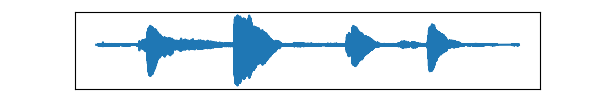
\includegraphics[width=0.62\textwidth]{./Chapter17/Figures/figure-hello-audio.png}};
\node[anchor=east,font=\scriptsize,align=center]  (a1) at  ([xshift=2.0em]input.west) {音频数据输入};
\node[minimum width=17.4em,minimum height=2.9em,draw=white,line width=3pt] at (0.3em,-0.02em){};

\node[anchor=north,draw,rounded corners=2pt,minimum width=16em, minimum height=2.2em,fill=yellow!20] (box) at ([xshift=0.4em]input.south){};
\node[anchor=west,minimum width=1.2em,minimum height=2.2em] (w1) at ([xshift=0.2em]box.west){{h}};
\node[anchor=west,minimum width=1.2em,minimum height=2.2em] (w2) at ([xshift=0.2em]w1.east){{e}};
\node[anchor=west,minimum width=1.2em,minimum height=2.2em] (w3) at ([xshift=0.2em]w2.east){{e}};
\node[anchor=west,minimum width=1.2em,minimum height=2.2em] (w4) at ([xshift=0.2em]w3.east){{$\epsilon$}};
\node[anchor=west,minimum width=1.2em,minimum height=2.2em] (w5) at ([xshift=0.2em]w4.east){{l}};
\node[anchor=west,minimum width=1.2em,minimum height=2.2em] (w6) at ([xshift=0.2em]w5.east){{$\epsilon$}};
\node[anchor=west,minimum width=1.2em,minimum height=2.2em] (w7) at ([xshift=0.2em]w6.east){{l}};
\node[anchor=west,minimum width=1.2em,minimum height=2.2em] (w8) at ([xshift=0.2em]w7.east){{l}};
\node[anchor=west,minimum width=1.2em,minimum height=2.2em] (w9) at ([xshift=0.2em]w8.east){{o}};
\node[anchor=west,minimum width=1.2em,minimum height=2.2em] (w10) at ([xshift=0.2em]w9.east){{o}};
\node[anchor=west,minimum width=1.2em,minimum height=2.2em] (w11) at ([xshift=0.2em]w10.east){{}};

\draw[very thick] (w1.south west) -- (w1.south east);
\draw[very thick] (w2.south west) -- (w2.south east);
\draw[very thick] (w3.south west) -- (w3.south east);
\draw[very thick] (w5.south west) -- (w5.south east);
\draw[very thick] (w7.south west) -- (w7.south east);
\draw[very thick] (w8.south west) -- (w8.south east);
\draw[very thick] (w9.south west) -- (w9.south east);
\draw[very thick] (w10.south west) -- (w10.south east);
%\draw[very thick] (w11.south west) -- (w11.south east);

\node[anchor=north,minimum width=1.2em,minimum height=1.4em,fill=gray!30] (m1) at ([yshift=-1em]w1.south){{h}};
\node[anchor=north,minimum width=2.64em,minimum height=1.4em,fill=gray!30] (m2) at ([yshift=-1em,xshift=0.72em]w2.south){{e}};
\node[anchor=north,minimum width=1.2em,minimum height=1.4em,fill=gray!30] (m3) at ([yshift=-1em]w4.south){};
\node[anchor=north,minimum width=1.2em,minimum height=1.4em,fill=gray!30] (m4) at ([yshift=-1em]w5.south){{l}};
\node[anchor=north,minimum width=1.2em,minimum height=1.4em,fill=gray!30] (m5) at ([yshift=-1em]w6.south){};
\node[anchor=north,minimum width=2.64em,minimum height=1.4em,fill=gray!30] (m6) at ([yshift=-1em,xshift=0.72em]w7.south){{l}};
\node[anchor=north,minimum width=2.64em,minimum height=1.4em,fill=gray!30] (m7) at ([yshift=-1em,xshift=0.72em]w9.south){{o}};
\node[anchor=north,minimum width=1.2em,minimum height=1.4em,fill=gray!30] (m8) at ([yshift=-1em]w11.south){};

\node[anchor=north,minimum width=1.2em,minimum height=1.4em,fill=gray!30] (o1) at ([yshift=-3.8em]w1.south){{h}};
\node[anchor=north,minimum width=1.2em,minimum height=1.4em,fill=gray!30] (o2) at ([yshift=-3.8em]w2.south){{e}};
\node[anchor=north,minimum width=1.2em,minimum height=1.4em,fill=gray!30] (o3) at ([yshift=-3.8em]w3.south){{l}};
\node[anchor=north,minimum width=1.2em,minimum height=1.4em,fill=gray!30] (o4) at ([yshift=-3.8em]w4.south){{l}};
\node[anchor=north,minimum width=1.2em,minimum height=1.4em,fill=gray!30] (o5) at ([yshift=-3.8em]w5.south){{o}};
\node[anchor=north,minimum width=1.2em,minimum height=1.4em,fill=gray!30] (o6) at ([yshift=-3.8em]w6.south){};
\node[anchor=north,minimum width=1.2em,minimum height=1.4em,fill=gray!30] at ([yshift=-3.8em]w7.south){};
\node[anchor=north,minimum width=1.2em,minimum height=1.4em,fill=gray!30] at ([yshift=-3.8em]w8.south){};
\node[anchor=north,minimum width=1.2em,minimum height=1.4em,fill=gray!30] at ([yshift=-3.8em]w9.south){};
\node[anchor=north,minimum width=1.2em,minimum height=1.4em,fill=gray!30] at ([yshift=-3.8em]w10.south){};
\node[anchor=north,minimum width=1.2em,minimum height=1.4em,fill=gray!30] at ([yshift=-3.8em]w11.south){};

\draw[blue!40,fill=blue!30,opacity=0.7] (w1.south west) -- (w1.south east) -- (o1.south east) -- (o1.south west) -- (w1.south west);
\draw[blue!40,fill=blue!30,opacity=0.7] (w2.south west) -- (w3.south east) -- (m2.south east) .. controls ([yshift=-0.3em]m2.south east) and ([yshift=0.3em]o2.north east) .. (o2.north east) -- (o2.south east) -- (o2.south west) -- (w2.south west);
\draw[blue!40,fill=blue!30,opacity=0.7] (w5.south west) -- (w5.south east) -- (m4.south east) .. controls ([yshift=-0.3em]m4.south east) and ([yshift=0.3em]o3.north east) .. (o3.north east) -- (o3.south east) -- (o3.south west) -- (o3.north west) .. controls ([yshift=0.3em]o3.north west) and ([yshift=-0.3em]m4.south west) .. (m4.south west) -- (w5.south west);
\draw[blue!40,fill=blue!30,opacity=0.7] (w7.south west) -- (w8.south east) -- (m6.south east) .. controls ([yshift=-0.3em]m6.south east) and ([yshift=0.3em]o4.north east) .. (o4.north east) -- (o4.south east) -- (o4.south west) -- (o4.north west) .. controls ([yshift=0.3em]o4.north west) and ([yshift=-0.3em]m6.south west) .. (m6.south west) -- (w7.south west);
\draw[blue!40,fill=blue!30,opacity=0.7] (w9.south west) -- (w10.south east) -- (m7.south east) .. controls ([yshift=-0.1em]m7.south east) and ([yshift=0.2em]o5.north east) .. (o5.north east) -- (o5.south east) -- (o5.south west) -- (o5.north west) .. controls ([yshift=0.1em]o5.north west) and ([yshift=-0.5em]m7.south west) .. (m7.south west) -- (w9.south west);
%\draw[blue!40,fill=blue!30,opacity=0.7] (w11.south west) -- (w11.south east) -- (m8.south east) .. controls ([yshift=-0.4em]m8.south east) and ([yshift=0.1em]o6.north east) .. (o6.north east) -- (o6.south east) -- (o6.south west) -- (o6.north west) .. controls ([yshift=0.1em]o6.north west) and ([yshift=-0.5em]m8.south west) .. (m8.south west) -- (w11.south west);

\node[anchor=north,font=\scriptsize,align=center] (a2) at  ([yshift=-1.4em]a1.south) {预测字母序列};
\node[anchor=north,font=\scriptsize,align=center] (a3) at  ([yshift=-1.8em]a2.south) {合并重复字母 \\ 并丢弃$\epsilon$};
\node[anchor=north,font=\scriptsize,align=center] (a4) at  ([yshift=-0.6em]a3.south) {最终结果输出};
\end{tikzpicture}
\caption{CTC预测单词序列示例}
\label{fig:17-8}
\end{figure}
%----------------------------------------------------------------------------------------------------

\parinterval CTC的一些特性使其可以很好的完成输入输出之间的对齐,例如:

%----------------------------------------------------------------------------------------------------
\begin{itemize}
    \vspace{0.5em}
    \item {\small\bfnew{输入和输出之间的对齐是单调的}}。对于音频输入序列$\{ s_1,...,s_m \} $,其对应的预测输出序列为$\{x_1,...,x_n \} $。假设$s_i$对应的预测输出结果为$x_j$,那么$s_{i+1}$相对应的预测结果只能是$x_j$、$x_{j+1}$和$\epsilon$三者中的一个。例如对于图\ref{fig:17-8}中的例子,如果输入的位置$s_i$已经对齐了字符“e”,那么$s_{i+1}$的对齐结果只能是“e”、“l”和$\epsilon$三者中的一个。
    \vspace{0.5em}
    \item {\small\bfnew{输入和输出之间是多对一的关系}}。也就是多个输入会对应到同一个输出上。这对于语音序列来说是非常自然的一件事情,由于输入的每个位置只包含非常短的语音特征,因此多个输入才可以对应到一个输出字符。
    \vspace{0.5em}
\end{itemize}
%----------------------------------------------------------------------------------------------------

\parinterval 将CTC应用到语音翻译中的方法非常简单,只需要在编码器的顶层加上一个额外的输出层即可(图\ref{fig:17-9})。通过这种方式,不需要增加过多的参数,就可以给模型加入一个较强的监督信息。

%----------------------------------------------------------------------------------------------------
\begin{figure}[htp]
\centering
\begin{tikzpicture}
	\tikzstyle{layer}=[draw,rounded corners=2pt,font=\scriptsize,align=center,minimum width=7.1em]
	\tikzstyle{word}=[font=\scriptsize]
%%%%encoder
\node[layer,fill=red!20] (en_sa) at (0,0){Multi-Head \\ Attention};
\node[anchor=south,layer,fill=yellow!20](en_add1) at ([yshift=1.0em]en_sa.north) {Add \& LayerNorm};
\node[layer,anchor=south,fill=green!20] (en_ffn) at ([yshift=1.0em]en_add1.north){Feed Forward \\ Network};
\node[anchor=south,layer,fill=yellow!20](en_add2) at ([yshift=1.0em]en_ffn.north) {Add \& LayerNorm};
\node[layer,anchor=south,fill=blue!20] (en_sf) at ([yshift=2.4em]en_add2.north){Softmax};
\node[draw,circle,inner sep=0pt, minimum size=1em,anchor=north,thick] (en_add) at ([yshift=-1.4em]en_sa.south){};
\draw[thick] (en_add.90) -- (en_add.-90);
\draw[thick] (en_add.0) -- (en_add.180);
\node[layer,anchor=north,fill=yellow!20] (en_cnn) at ([yshift=-1.0em]en_add.south){CNN};
\node[anchor=east,font=\scriptsize,align=center] (en_pos) at ([xshift=-2em]en_add.west){位置编码};
\node[anchor=north,font=\scriptsize,align=center] (en_input) at ([yshift=-1em]en_cnn.south){源语言语音特征\\(FBank/MFCC)};

\draw[->,thick] (en_input.90) -- ([yshift=-0.1em]en_cnn.-90);
\draw[->,thick] ([yshift=0.1em]en_cnn.90) -- ([yshift=-0.1em]en_add.-90);
\draw[->,thick] ([yshift=0.1em]en_add.90) -- ([yshift=-0.1em]en_sa.-90);
\draw[->,thick] ([yshift=0.1em]en_sa.90) -- ([yshift=-0.1em]en_add1.-90);
\draw[->,thick] ([yshift=0.1em]en_add1.90) -- ([yshift=-0.1em]en_ffn.-90);
\draw[->,thick] ([yshift=0.1em]en_ffn.90) --([yshift=-0.1em]en_add2.-90);
\draw[->,thick] ([yshift=0.1em]en_add2.90) -- ([yshift=-0.1em]en_sf.-90);
\draw[->,thick] ([yshift=0.1em]en_sf.90) -- ([yshift=1.5em]en_sf.90)node[left,pos=0.5]{\scriptsize{CTC Loss}};
\draw[->,rounded corners=2pt,thick] ([yshift=-0.6em]en_sa.south)--([yshift=-0.6em,xshift=-4.0em]en_sa.south)--([xshift=-0.43em]en_add1.west)--(en_add1.west);
\draw[->,rounded corners=2pt,thick] ([yshift=-0.6em]en_ffn.south)--([yshift=-0.6em,xshift=-4.0em]en_ffn.south)--([xshift=-0.43em]en_add2.west)--(en_add2.west);

%%%%decoder
\node[draw,circle,inner sep=0pt, minimum size=1em,anchor=west,thick] (de_add) at ([xshift=9em]en_add.east){};
\draw[thick] (de_add.90) -- (de_add.-90);
\draw[thick] (de_add.0) -- (de_add.180);
\node[layer,anchor=south,fill=red!20] (de_sa) at ([yshift=1.4em]de_add.north){Masked \\Multi-Head\\Attention};
\node[anchor=south,layer,fill=yellow!20](de_add1) at ([yshift=1.0em]de_sa.north) {Add \& LayerNorm};
\node[layer,anchor=south,fill=red!20] (de_ca) at ([yshift=1.0em]de_add1.north){Multi-Head \\ Attention};
\node[anchor=south,layer,fill=yellow!20](de_add2) at ([yshift=1.0em]de_ca.north) {Add \& LayerNorm};
\node[layer,anchor=south,fill=green!20] (de_ffn) at ([yshift=1.0em]de_add2.north){Feed Forward \\ Network};
\node[anchor=south,layer,fill=yellow!20](de_add3) at ([yshift=1.0em]de_ffn.north) {Add \& LayerNorm};
\node[layer,anchor=south,fill=blue!20] (sf) at ([yshift=1.2em]de_add3.north){Softmax};
\node[anchor=north,font=\scriptsize,align=center] (de_input) at ([yshift=-1.1em]de_add.south){目标语言文本\\编码表示};

\node[anchor=west,font=\scriptsize,align=center] (de_pos) at ([xshift=2em]de_add.east){位置编码};

\draw[->,thick] (de_input.90) -- ([yshift=-0.1em]de_add.-90);
\draw[->,thick] ([yshift=0.1em]de_add.90) -- ([yshift=-0.1em]de_sa.-90);
\draw[->,thick] ([yshift=0.1em]de_sa.90) -- ([yshift=-0.1em]de_add1.-90);
\draw[->,thick] ([yshift=0.1em]de_add1.90) -- ([yshift=-0.1em]de_ca.-90);
\draw[->,thick] ([yshift=0.1em]de_ca.90) -- ([yshift=-0.1em]de_add2.-90);
\draw[->,thick] ([yshift=0.1em]de_add2.90) -- ([yshift=-0.1em]de_ffn.-90);
\draw[->,thick] ([yshift=0.1em]de_ffn.90) -- ([yshift=-0.1em]de_add3.-90);
\draw[->,thick] ([yshift=0.1em]de_add3.90) -- ([yshift=-0.1em]sf.-90);
\draw[->,thick] ([yshift=0.1em]sf.90) -- ([yshift=1.0em]sf.90);
\draw[->,thick] ([xshift=0.1em]en_pos.0) -- ([xshift=-0.1em]en_add.180);
\draw[->,thick] ([xshift=-0.1em]de_pos.180) -- ([xshift=0.1em]de_add.0);
\draw[->,rounded corners=2pt,thick] ([yshift=-0.6em]de_sa.south)--([yshift=-0.6em,xshift=4.0em]de_sa.south)--([xshift=0.43em]de_add1.east)--(de_add1.east);
\draw[->,rounded corners=2pt,thick] ([yshift=-0.6em]de_ca.south)--([yshift=-0.6em,xshift=4.0em]de_ca.south)--([xshift=0.43em]de_add2.east)--(de_add2.east);
\draw[->,rounded corners=2pt,thick] ([yshift=-0.6em]de_ffn.south)--([yshift=-0.6em,xshift=4.0em]de_ffn.south)--([xshift=0.43em]de_add3.east)--(de_add3.east);

\draw[->,rounded corners=2pt,thick] ([yshift=0.1em]en_add2.90) -- ([yshift=1.5em]en_add2.90) -- ([xshift=5.0em,yshift=1.5em]en_add2.90) -- ([xshift=-1.5em]de_ca.west) -- ([xshift=-0.1em]de_ca.west);


\begin{pgfonlayer}{background}
\node[draw=ugreen,rounded corners=2pt,inner xsep=6pt,inner ysep=8pt,dashed,thick,xshift=-0.2em,yshift=-0.2em][fit=(en_add1)(en_add2)(en_sa)(en_ffn)](box1){};
\node[draw=red,rounded corners=2pt,inner xsep=6pt,inner ysep=8pt,dashed,thick,xshift=0.2em,yshift=-0.2em][fit=(de_sa)(de_ca)(de_ffn)(de_add3)](box2){};
\end{pgfonlayer}

\node[anchor=east,font=\scriptsize,text=ugreen] at ([xshift=-0.1em]box1.west){$N \times$};
\node[anchor=west,font=\scriptsize,text=red] at ([xshift=0.1em]box2.east){$\times N$};
\node[anchor=east,font=\scriptsize] at ([xshift=-0.1em]en_cnn.west){$2 \times$};
\node[anchor=east,font=\scriptsize,align=center,text=ugreen] at ([xshift=-0.1em,yshift=3em]box1.west){ST \\ 编码器};
\node[anchor=west,font=\scriptsize,align=center,text=red] at ([xshift=0.1em,yshift=5em]box2.east){ST \\ 解码器};
\end{tikzpicture}
\caption{基于CTC的语音翻译模型}
\label{fig:17-9}
\end{figure}
%----------------------------------------------------------------------------------------------------

\parinterval 另外一种多任务学习的思想是通过两个解码器,分别预测语音对应的源语言句子和目标语言句子,具体有图\ref{fig:17-10}展示的三种方式\upcite{DBLP:conf/naacl/AnastasopoulosC18,DBLP:conf/asru/BaharBN19}。图\ref{fig:17-10}(a)中采用单编码器-双解码器的方式,两个解码器根据编码器的表示,分别预测源语言句子和目标语言句子,从而使编码器训练地更加充分。这种做法的好处在于源语言的文本生成任务可以辅助翻译过程,相当于为源语言语音提供了额外的“模态”信息。图\ref{fig:17-10}(b)则通过使用两个级联的解码器,先利用第一个解码器生成源语言句子,然后再利用第一个解码器的表示,通过第二个解码器生成目标语言句子。这种方法通过增加一个中间输出,降低了模型的训练难度,但同时也会带来额外的解码耗时,因为两个解码器需要串行地进行生成。图\ref{fig:17-10}(c) 中模型更进一步,第二个编码器联合编码器和第一个解码器的表示进行生成,更充分地利用了已有信息。
%----------------------------------------------------------------------------------------------------
\begin{figure}[htp]
\centering
\tikzstyle{coder} = [rectangle,thick,rounded corners,minimum height=2.2em,minimum width=4.3em,text centered,draw=black,fill=red!20]

\begin{tikzpicture}[node distance = 0,scale = 0.75]
\tikzstyle{every node}=[scale=0.75]

\node(encoder)[coder]at (0,0){\large{编码器}};
\node(decoder_1)[coder,above of =encoder,xshift=-1.6cm,yshift=2.8cm,fill=blue!20]{\large{解码器}};
\node(decoder_2)[coder,above of =encoder, xshift=1.6cm,yshift=2.8cm,fill=yellow!20]{\large{解码器}};
\node(s)[below of = encoder,yshift=-1.8cm,scale=1.2]{$s$};
\node(x)[above of = decoder_1,yshift=1.8cm,scale=1.2]{$x$};
\node(y)[above of = decoder_2,yshift=1.8cm,scale=1.2]{$y$};

\draw[->,thick](s.north)to(encoder.south);
\draw[->,thick](decoder_1.north)to(x.south);
\draw[->,thick](decoder_2.north)to(y.south);
\draw[->,thick](encoder.north)--([yshift=0.7cm]encoder.north)--([xshift=-4.16em,yshift=0.7cm]encoder.north)--(decoder_1.south);
\draw[->,thick](encoder.north)--([yshift=0.7cm]encoder.north)--([xshift=4.16em,yshift=0.7cm]encoder.north)--(decoder_2.south);
\node [anchor=north,scale = 1.2](pos1) at (s.south) {(a) 单编码器-双解码器};
\node [anchor=south,scale=1.2] (node1) at ([xshift=-2.0em,yshift=9em]decoder_1.north) {{$x$:源语言文本数据}};
\node [anchor=north,scale=1.2] (node2) at ([xshift=0.63em]node1.south){{$y$:目标语言文本数据}};
\node [anchor=north,scale=1.2] (node3) at ([xshift=-0.57em]node2.south){{$s$:源语言语音数据}};
%%%%%%%%%%%%%%%%%%%%%%%%级联
\node(encoder-2)[coder]at ([xshift=12.0em]encoder.east){\large{编码器}};
\node(decoder_1-2)[coder,above of =encoder-2,yshift=1.4cm,fill=blue!20]{\large{解码器}};
\node(decoder_2-2)[coder,above of =decoder_1-2, yshift=1.4cm,fill=yellow!20]{\large{解码器}};
\node(s-2)[below of = encoder-2,yshift=-1.8cm,scale=1.2]{$s$};
\node(y-2)[above of = decoder_2-2,yshift=1.8cm,scale=1.2]{$y$};

\draw[->,thick](s-2.north)to(encoder-2.south);
\draw[->,thick](encoder-2.north)to(decoder_1-2.south);
\draw[->,thick](decoder_1-2.north)to(decoder_2-2.south);
\draw[->,thick](decoder_2-2.north)to(y-2.south);
\node [anchor=north,scale = 1.2](pos2) at (s-2.south) {(b) 级联解码器};
%%%%%%%%%%%%%%%%%%%%%%%%联合
\node(encoder-3)[coder]at([xshift=10.0em]encoder-2.east){\large{编码器}};
\node(decoder_1-3)[coder,above of =encoder-3,xshift=-1.6cm,yshift=2.8cm,fill=blue!20]{\large{解码器}};
\node(decoder_2-3)[coder,above of =encoder-3, xshift=1.6cm,yshift=2.8cm,fill=yellow!20]{\large{解码器}};
\node(s-3)[below of = encoder-3,yshift=-1.8cm,scale=1.2]{$s$};
\node(y-3)[above of = decoder_2-3,yshift=1.8cm,scale=1.2]{$y$};

\draw[->,thick](s-3.north)to(encoder-3.south);
\draw[->,thick](decoder_1-3.east)to(decoder_2-3.west);
\draw[->,thick](decoder_2-3.north)to(y-3.south);
\draw[->,thick](encoder-3.north)--([yshift=0.7cm]encoder-3.north)--([xshift=-4.16em,yshift=0.7cm]encoder-3.north)--(decoder_1-3.south);
\draw[->,thick](encoder-3.north)--([yshift=0.7cm]encoder-3.north)--([xshift=4.16em,yshift=0.7cm]encoder-3.north)--(decoder_2-3.south);
\node [anchor=north,scale = 1.2](pos3) at (s-3.south) {(c) 联合编解码器};
\end{tikzpicture}
\caption{双解码器进行语音翻译的三种方式}
\label{fig:17-10}
\end{figure}
%----------------------------------------------------------------------------------------------------

%----------------------------------------------------------------------------------------
%    NEW SUBSUB-SECTION
%----------------------------------------------------------------------------------------
\subsubsection{2. 迁移学习}

\parinterval 相比语音识别和文本翻译,端到端语音翻译的训练数据量要小很多,因此,如何利用其它数据来增加可用的数据量是语音翻译的一个重要方向。和文本翻译中的方法相似,一种思路是利用迁移学习或预训练,利用其他语言的双语数据预训练模型参数,然后迁移到生成目标语言的任务上\upcite{DBLP:conf/naacl/BansalKLLG19},或者是利用语音识别数据或文本翻译数据,分别预训练编码器和解码器的参数,用于初始化语音翻译模型的参数\upcite{DBLP:conf/icassp/BerardBKP18}。预训练的编码器对语音翻译模型的学习尤为重要\upcite{DBLP:conf/naacl/BansalKLLG19},相比文本数据,语音数据的复杂性更高,仅使用小规模语音翻译数据很难学习充分。此外,模型对声学特征的学习与语言并不是强相关的,其他语种预训练的编码器对模型学习也是有帮助的。

%----------------------------------------------------------------------------------------
%    NEW SUBSUB-SECTION
%----------------------------------------------------------------------------------------
\subsubsection{3. 数据增强}

\parinterval 数据增强是增加训练数据最直接的一种方法。不同于文本翻译的回译等方法(见{\chaptersixteen}),语音翻译并不具有简单的“可逆性”。如果要利用回译的思想,需要通过一个模型,将目标语言文本转化为源语言语音,但实际上这种模型是不能简单得到的。因此,一个简单的思路是通过一个反向翻译模型和语音合成模型级联来生成伪数据\upcite{DBLP:conf/icassp/JiaJMWCCALW19}。 另外,正向翻译模型生成的伪数据在文本翻译中也被验证了对模型训练有一定的帮助,因此同样可以利用语音识别和文本翻译模型,将源语言语音翻译成目标语言文本,得到伪平行语料。

%----------------------------------------------------------------------------------------------------

\parinterval 此外,也可以利用在海量的无标注语音数据上预训练的{\small\bfnew{自监督}}\index{自监督}(Self-supervised)\index{Self-supervised}模型作为一个特征提取器,将从语音中提取的特征作为语音翻译模型的输入,可以有效提高模型的性能\upcite{DBLP:conf/interspeech/WuWPG20}。相比语音翻译模型,文本翻译模型任务更加简单,因此一种思想是利用文本翻译模型来指导语音翻译模型,比如,使用知识蒸馏\upcite{DBLP:conf/interspeech/LiuXZHWWZ19}、正则化\upcite{DBLP:conf/emnlp/AlinejadS20}等方法。为了简化语音翻译模型的学习,也可以使用课程学习方法(见{\chapterthirteen})。这样,使模型从语音识别任务,逐渐过渡到语音翻译任务,这种由易到难的训练策略可以使模型训练更加充分\upcite{DBLP:journals/corr/abs-1802-06003,DBLP:conf/acl/WangWLZY20}。

%----------------------------------------------------------------------------------------
%    NEW SECTION
%----------------------------------------------------------------------------------------
\sectionnewpage
\section{图像翻译}

\parinterval 在人类所接受的信息中,视觉信息的比重往往不亚于语音和文本信息,甚至更多。视觉信息通常以图像的形式存在,近几年,结合图像的多模态机器翻译受到了广泛的关注。多模态机器翻译(图\ref{fig:17-11} (a))简单来说就是结合源语言和其他模态(例如图像等)的信息生成目标语言的过程。这种结合图像的机器翻译还是一种狭义上的“翻译”,它本质上还是从源语言到目标语言或者说从文本到文本的翻译。事实上从图像到文本(图\ref{fig:17-11}(b))的转换,即给定图像,生成与图像内容相关的描述,也可以被称为广义上的“翻译”。例如,{\small\bfnew{图片描述生成}}\index{图片描述生成}(Image Captioning)\index{Image Captioning}就是一种典型的图像到文本的翻译。当然,这种广义上的翻译形式不仅仅包括图像到文本的转换,还可以包括从图像到图像的转换(图\ref{fig:17-11}(c)),甚至是从文本到图像的转换(图\ref{fig:17-11}(d))等等。这里将这些与图像相关的翻译任务统称为图像翻译。

%----------------------------------------------------------------------------------------------------
\begin{figure}[htp]
\centering
\begin{tikzpicture}[scale=0.6]
\tikzstyle{every node}=[scale=0.6]
%figure 1
\coordinate (A1) at (0, 0);
\coordinate (B1) at ([xshift=1.5em,yshift=-0.4em]A1);
\coordinate (C1) at ([xshift=0.3em,yshift=-2.6em]A1);
\coordinate (D1) at ([xshift=2.7em,yshift=-2.6em]A1);
\coordinate (E1) at ([xshift=2.4em,yshift=-1.5em]A1);
\coordinate (F1) at ([xshift=0.3em]D1);

\coordinate (G1) at ([xshift=0.3em,yshift=-5em]A1);
\coordinate (H1) at ([xshift=0.4em,yshift=-1.6em]G1);
\coordinate (I1) at ([xshift=0.4em,yshift=-2.0em]G1);
\coordinate (J1) at ([xshift=0.4em,yshift=-2.5em]G1);
\coordinate (K1) at ([xshift=0.4em,yshift=-3.0em]G1);
\coordinate (L1) at ([xshift=0.4em,yshift=-3.5em]G1);

\coordinate (G2) at ([xshift=8em,yshift=-2.5em]A1);
\coordinate (H2) at ([xshift=0.4em,yshift=-1.6em]G2);
\coordinate (I2) at ([xshift=0.4em,yshift=-2.0em]G2);
\coordinate (J2) at ([xshift=0.4em,yshift=-2.5em]G2);
\coordinate (K2) at ([xshift=0.4em,yshift=-3.0em]G2);
\coordinate (L2) at ([xshift=0.4em,yshift=-3.5em]G2);

%figure 2
\coordinate (A2) at ([yshift=-0.5em,xshift=7em]G2);
\coordinate (B2) at ([xshift=1.5em,yshift=-0.4em]A2);
\coordinate (C2) at ([xshift=0.3em,yshift=-2.6em]A2);
\coordinate (D2) at ([xshift=2.7em,yshift=-2.6em]A2);
\coordinate (E2) at ([xshift=2.4em,yshift=-1.5em]A2);
\coordinate (F2) at ([xshift=0.3em]D2);

\coordinate (G3) at ([xshift=8em,yshift=0.5em]A2);
\coordinate (H3) at ([xshift=0.4em,yshift=-1.6em]G3);
\coordinate (I3) at ([xshift=0.4em,yshift=-2.0em]G3);
\coordinate (J3) at ([xshift=0.4em,yshift=-2.5em]G3);
\coordinate (K3) at ([xshift=0.4em,yshift=-3.0em]G3);
\coordinate (L3) at ([xshift=0.4em,yshift=-3.5em]G3);

%figure 3
\coordinate (A3) at ([yshift=-0.5em,xshift=7em]G3);
\coordinate (B3) at ([xshift=1.5em,yshift=-0.4em]A3);
\coordinate (C3) at ([xshift=0.3em,yshift=-2.6em]A3);
\coordinate (D3) at ([xshift=2.7em,yshift=-2.6em]A3);
\coordinate (E3) at ([xshift=2.4em,yshift=-1.5em]A3);
\coordinate (F3) at ([xshift=0.3em]D3);

\coordinate (A4) at ([xshift=8em]A3);
\coordinate (B4) at ([xshift=1.5em,yshift=-0.4em]A4);
\coordinate (C4) at ([xshift=0.3em,yshift=-2.6em]A4);
\coordinate (D4) at ([xshift=2.7em,yshift=-2.6em]A4);
\coordinate (E4) at ([xshift=2.4em,yshift=-1.5em]A4);
\coordinate (F4) at ([xshift=0.3em]D4);

%figure 4
\coordinate (G4) at ([xshift=7.6em,yshift=0.5em]A4);
\coordinate (H4) at ([xshift=0.4em,yshift=-1.6em]G4);
\coordinate (I4) at ([xshift=0.4em,yshift=-2.0em]G4);
\coordinate (J4) at ([xshift=0.4em,yshift=-2.5em]G4);
\coordinate (K4) at ([xshift=0.4em,yshift=-3.0em]G4);
\coordinate (L4) at ([xshift=0.4em,yshift=-3.5em]G4);

\coordinate (A5) at ([yshift=-0.5em,xshift=8em]G4);
\coordinate (B5) at ([xshift=1.5em,yshift=-0.4em]A5);
\coordinate (C5) at ([xshift=0.3em,yshift=-2.6em]A5);
\coordinate (D5) at ([xshift=2.7em,yshift=-2.6em]A5);
\coordinate (E5) at ([xshift=2.4em,yshift=-1.5em]A5);
\coordinate (F5) at ([xshift=0.3em]D5);

\foreach \x in {1,2,3,4,5}{
\draw[-,line width=2pt] (A\x) -- ([xshift=3.6em]A\x) -- ([xshift=3.6em,yshift=-3em]A\x) -- ([yshift=-3em]A\x) -- (A\x) -- ([xshift=1em]A\x);
\draw[-, very thick] (B\x) -- (C\x) -- (D\x) -- (B\x);
\draw[-, very thick,fill=black] ([xshift=-0.6em,yshift=-1.2em]B\x)  -- ([xshift=-0.3em,yshift=-1em]B\x) -- ([yshift=-1.2em]B\x) --([xshift=0.3em,yshift=-1em]B\x) -- ([xshift=0.6em,yshift=-1.2em]B\x) -- (D\x) -- (C\x) -- ([xshift=-0.6em,yshift=-1.2em]B\x);
\draw[-, very thick,fill=black] (E\x) -- ([xshift=0.2em,yshift=0.3em]E\x) -- ([xshift=0.33em]F\x) -- (F\x) -- (E\x);
\node[circle,inner sep=0pt,minimum size=0.4em,fill=black] at ([xshift=-0.7em,yshift=-0.2em]B\x){};
}

\foreach \y in {1,2,3,4}{
\draw[-,line width=2pt] (G\y) -- ([xshift=1.6em]G\y) -- ([xshift=3em,yshift=-1.4em]G\y) -- ([xshift=3em,yshift=-4em]G\y) -- ([yshift=-4em]G\y) -- (G\y) -- ([xshift=1em]G\y);
\draw[-,line width=2pt] ([xshift=1.6em]G\y) -- ([xshift=1.5em,yshift=-1.4em]G\y) -- ([xshift=3em,yshift=-1.4em]G\y) ;
\draw[-,line width=1.6pt] (H\y) -- ([xshift=0.6em]H\y);
\draw[-,line width=1.6pt] (I\y) -- ([xshift=2em]I\y);
\draw[-,line width=1.6pt] (J\y) -- ([xshift=2em]J\y);
\draw[-,line width=1.6pt] (K\y) -- ([xshift=2em]K\y);
\draw[-,line width=1.6pt] (L\y) -- ([xshift=2em]L\y);
}

\draw[-,thick] ([yshift=4em,xshift=5em]G2) -- ([yshift=-8em,xshift=5em]G2);
\draw[-,thick] ([yshift=4em,xshift=5em]G3) -- ([yshift=-8em,xshift=5em]G3);
\draw[-,thick] ([yshift=4.5em,xshift=5.6em]A4) -- ([yshift=-7.5em,xshift=5.6em]A4);

\node [draw,single arrow,minimum height=2.4em,single arrow head extend=0.4em] (arrow1) at ([xshift=-2.4em,yshift=-2em]G2) {};
\node [draw,single arrow,minimum height=2.4em,single arrow head extend=0.4em] (arrow2) at ([xshift=-2.4em,yshift=-2em]G3) {};
\node [draw,single arrow,minimum height=2.4em,single arrow head extend=0.4em] (arrow3) at ([xshift=-2.4em,yshift=-1.5em]A4) {};
\node [draw,single arrow,minimum height=2.4em,single arrow head extend=0.4em] (arrow4) at ([xshift=-2.5em,yshift=-1.5em]A5) {};

\node[anchor=north,font=\small,scale=1.5] at ([yshift=-6em]arrow1.south){(a) 多模态机器翻译};
\node[anchor=north,font=\small,scale=1.5] at ([yshift=-6em]arrow2.south){(b) 图像到文本翻译};
\node[anchor=north,font=\small,scale=1.5] at ([yshift=-6em]arrow3.south){(c) 图像到图像翻译};
\node[anchor=north,font=\small,scale=1.5] at ([yshift=-6em]arrow4.south){(d) 文本到图像翻译};
\end{tikzpicture}
%------------------------------------------------------------------------------------------------------------


\caption{图像翻译任务}
\label{fig:17-11}
\end{figure}
%----------------------------------------------------------------------------------------------------

%----------------------------------------------------------------------------------------
%    NEW SUB-SECTION
%----------------------------------------------------------------------------------------

\subsection{基于图像增强的文本翻译}
\label{sec:image-augmented-translation}

\parinterval 在文本翻译中引入图像信息是最典型的多模态机器翻译任务。虽然多模态机器翻译还是一种从源语言文本到目标语言文本的转换,但是在转换的过程中,融入了其他模态的信息减少了歧义的产生。例如前文提到的通过与源语言相关的图像信息,将“A girl jumps off a bank .”中“bank”翻译为“河岸”而不是“银行”,因为图像中出现了河岸,因此“bank”的歧义大大降低。换句话说,对于同一图像或者视觉场景的描述,源语言和目标语言描述的信息是一致的,只不过,体现在不同语言上会有表达方法上的差异。那么,图像就会存在一些源语言和目标语言的隐含对齐“约束”,而这种“约束”可以捕捉语言中不易表达的隐含信息。

\parinterval 如何融入视觉信息,更好的理解多模态上下文语义是多模态机器翻译研究的重点\upcite{DBLP:conf/wmt/SpeciaFSE16,DBLP:conf/wmt/CaglayanABGBBMH17,DBLP:conf/wmt/LibovickyHTBP16},主要方向包括基于特征融合的方法\upcite{DBLP:conf/emnlp/CalixtoL17,DBLP:journals/corr/abs-1712-03449,DBLP:conf/wmt/HelclLV18}、基于联合模型的方法\upcite{DBLP:conf/ijcnlp/ElliottK17,DBLP:conf/acl/YinMSZYZL20}。下面是具体介绍。

%----------------------------------------------------------------------------------------
%    NEW SUBSUB-SECTION
%----------------------------------------------------------------------------------------

\subsubsection{1. 基于特征融合的方法}

\parinterval 早期,通常将图像信息作为输入句子的一部分\upcite{DBLP:conf/emnlp/CalixtoL17,DBLP:conf/wmt/HuangLSOD16},或者用其对编码器、解码器的状态进行初始化\upcite{DBLP:conf/emnlp/CalixtoL17,Elliott2015MultilingualID,DBLP:conf/wmt/MadhyasthaWS17}。如图\ref{fig:17-12}所示,图中$y_{<}$表示当前时刻之前的单词序列,对图像特征的提取通常是基于卷积神经网络,有关卷积神经网络的内容,可以参考{\chaptereleven}内容。通过卷积神经网络得到全局图像特征,在进行维度变换后,将其作为源语言输入的一部分或者初始化状态引入到模型当中。但是,这种图像信息的引入方式有以下两个缺点:

\begin{itemize}
    \vspace{0.5em}
    \item 图像信息不全都是有用的,往往存在一些与源语言或目标语言无关的信息,作为全局特征会引入噪音。
    \vspace{0.5em}
    \item 图像信息作为源语言的一部分或者初始化状态,间接地参与了译文的生成,在神经网络的计算过程中,图像信息会有一定的损失。
    \vspace{0.5em}
\end{itemize}

%----------------------------------------------------------------------------------------------------
\begin{figure}[htp]
\centering
\begin{tikzpicture}[scale=0.8]
\tikzstyle{every node}=[scale=0.8]
%figure 1
\coordinate (A1) at (0, 0);
\coordinate (B1) at ([xshift=1.5em,yshift=-0.4em]A1);
\coordinate (C1) at ([xshift=0.3em,yshift=-2.6em]A1);
\coordinate (D1) at ([xshift=2.7em,yshift=-2.6em]A1);
\coordinate (E1) at ([xshift=2.4em,yshift=-1.5em]A1);
\coordinate (F1) at ([xshift=0.3em]D1);


%figure 2
\coordinate (A2) at ([xshift=15em]A1);
\coordinate (B2) at ([xshift=1.5em,yshift=-0.4em]A2);
\coordinate (C2) at ([xshift=0.3em,yshift=-2.6em]A2);
\coordinate (D2) at ([xshift=2.7em,yshift=-2.6em]A2);
\coordinate (E2) at ([xshift=2.4em,yshift=-1.5em]A2);
\coordinate (F2) at ([xshift=0.3em]D2);


\foreach \x in {1,2}{
\draw[-,line width=2pt] (A\x) -- ([xshift=3.6em]A\x) -- ([xshift=3.6em,yshift=-3em]A\x) -- ([yshift=-3em]A\x) -- (A\x) -- ([xshift=1em]A\x);
\draw[-, very thick] (B\x) -- (C\x) -- (D\x) -- (B\x);
\draw[-, very thick,fill=black] ([xshift=-0.6em,yshift=-1.2em]B\x)  -- ([xshift=-0.3em,yshift=-1em]B\x) -- ([yshift=-1.2em]B\x) --([xshift=0.3em,yshift=-1em]B\x) -- ([xshift=0.6em,yshift=-1.2em]B\x) -- (D\x) -- (C\x) -- ([xshift=-0.6em,yshift=-1.2em]B\x);
\draw[-, very thick,fill=black] (E\x) -- ([xshift=0.2em,yshift=0.3em]E\x) -- ([xshift=0.33em]F\x) -- (F\x) -- (E\x);
\node[circle,inner sep=0pt,minimum size=0.4em,fill=black] at ([xshift=-0.7em,yshift=-0.2em]B\x){};
\node[draw,rounded corners=2pt,fill=yellow!20,minimum width=4.3em,minimum height=2.2em](cnn\x) at ([xshift=1.8em,yshift=3.6em]A\x){CNN};
}
\node[draw,anchor=south,rounded corners=2pt,minimum width=4.0cm,minimum height=2.2em,fill=red!20](encoder) at ([yshift=2.6em,xshift=2.2em]cnn1.north){编码器};
\node[anchor=north,font=\Large](x) at ([xshift=2.5em,yshift=-3.4em]encoder.south){$\seq{x}$};

\node[draw,anchor=south,rounded corners=2pt,minimum width=4.0cm,minimum height=2.2em,fill=blue!20](decoder) at ([yshift=2.6em,xshift=2.2em]cnn2.north){解码器};
\node[anchor=north,font=\Large](y) at ([xshift=2.5em,yshift=-3.4em]decoder.south){$\seq{y}_{<}$};
\node[anchor=south,font=\Large](y_1) at ([yshift=3em]decoder.north){$\seq{y}$};

\draw[->,thick] ([yshift=-2.1em]cnn1.south) -- ([yshift=-0.1em]cnn1.south);
\draw[->,thick] ([yshift=-2.1em]cnn2.south) -- ([yshift=-0.1em]cnn2.south);
\draw[->,thick] ([yshift=0.1em]cnn1.north) -- ([yshift=2.4em]cnn1.north);
\draw[->,thick] ([yshift=0.1em]cnn2.north) -- ([yshift=2.4em]cnn2.north);
\draw[->,thick] ([yshift=0.3em]x.north) -- ([yshift=4.5em]x.south);
\draw[->,thick] ([yshift=0.3em]y.north) -- ([yshift=4.7em]y.south);
\draw[->,thick] ([xshift=0.1em]encoder.east) -- ([xshift=-0.1em]decoder.west);
\draw[->,thick] ([yshift=0.1em]decoder.north) -- ([yshift=-0.1em]y_1.south);
\node [anchor=south,scale=1.2] (node1) at ([xshift=-0.7em,yshift=4em]encoder.north) {\small{$x$:源语言文本数据}};
\node [anchor=north,scale=1.2] (node2) at ([xshift=0.57em]node1.south){\small{$y$:目标语言文本数据}};
\end{tikzpicture}
%------------------------------------------------------------------------------------------------------------


\caption{基于全局视觉特征的多模态翻译方法}
\label{fig:17-12}
\end{figure}
%----------------------------------------------------------------------------------------------------

\parinterval 说到噪音问题就不得不提到注意力机制的引入,前面章节中提到过这样的一个例子:

\vspace{0.8em}
\centerline{中午/没/吃饭/,/又/刚/打/了/ 一/下午/篮球/,/我/现在/很/饿/ ,/我/想\underline{\quad \quad} 。}
\vspace{0.8em}

\parinterval 想在横线处填写“吃饭”,“吃东西”的原因是在读句子的过程中,关注到了“没/吃饭”,“很/饿”等关键息。这是在语言生成中注意力机制所解决的问题,即对于要生成的目标语言单词,相关性更高的语言片段应该更加“重要”,而不是将所有单词一视同仁。同样的,注意力机制也应用在多模态机器翻译中,即在生成目标单词时,更应该关注与目标单词相关的图像部分,而弱化对其他部分的关注。另外,注意力机制的引入,也使图像信息更加直接地参与目标语言的生成,解决了在不使用注意力机制的方法中图像信息传递损失的问题。

%----------------------------------------------------------------------------------------------------
\begin{figure}[htp]
\centering
\begin{tikzpicture}[node distance = 0,scale = 0.7]
\tikzstyle{every node}=[scale=0.7]
\node[draw=white] (input) at (0,0){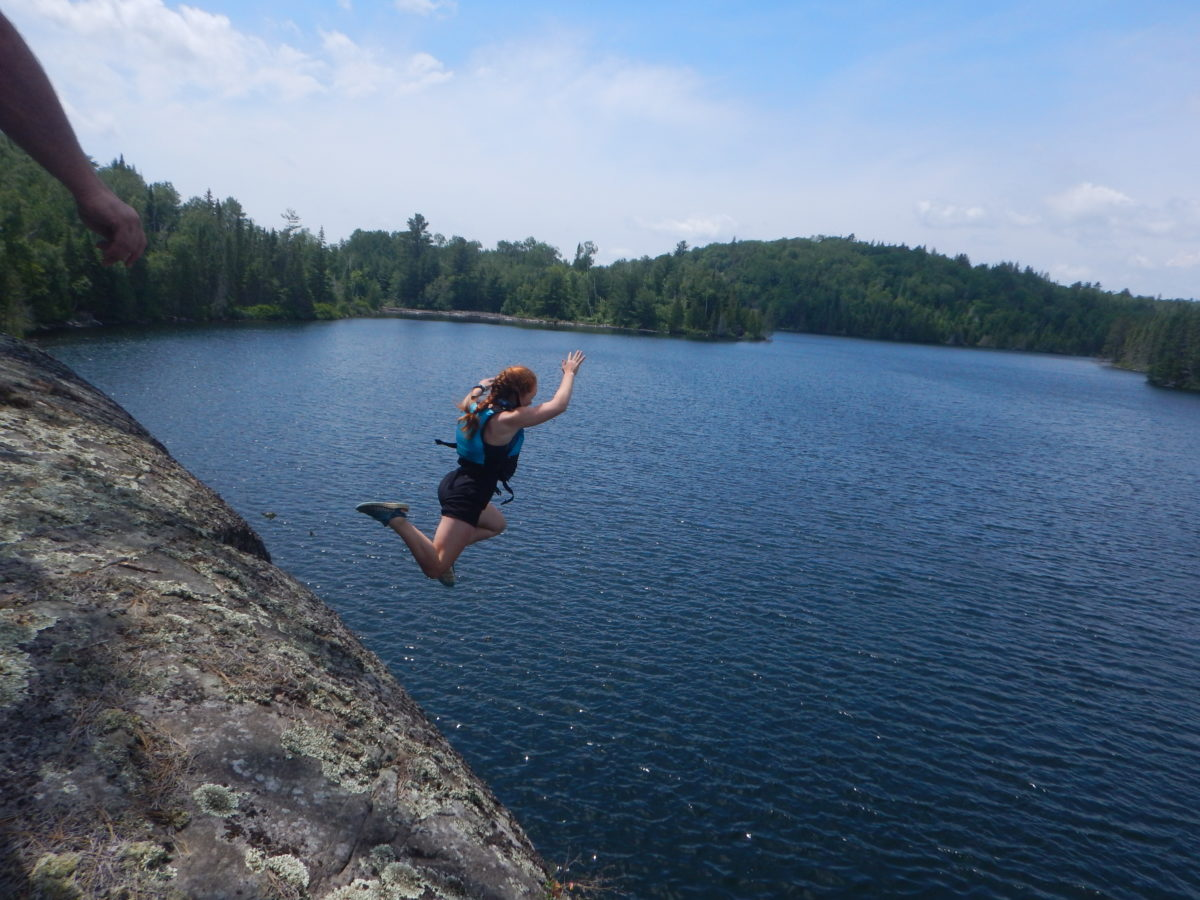
\includegraphics[width=0.62\textwidth]{./Chapter17/Figures/figure-bank-without-attention.jpg}};(1.9,-1.4);
\node[draw=white] (input) at (10,0){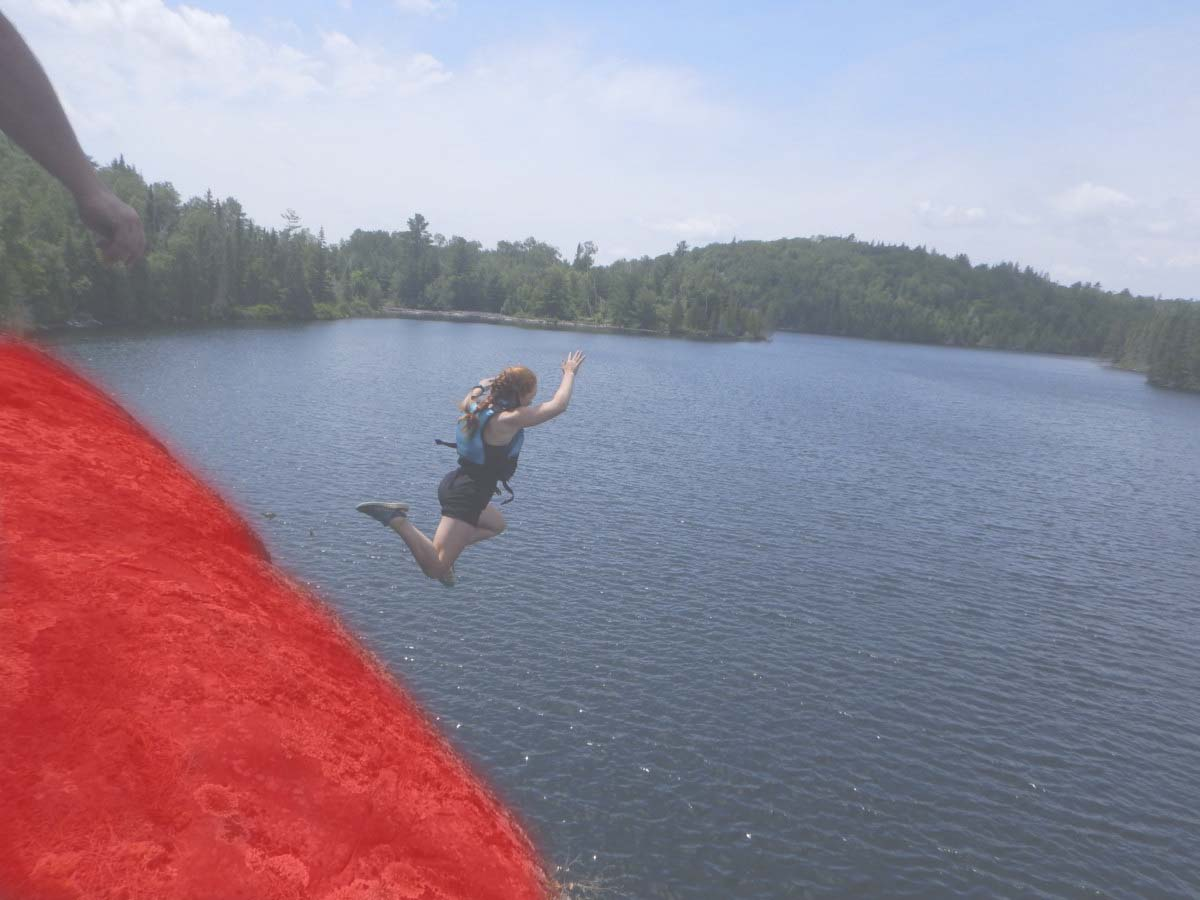
\includegraphics[width=0.62\textwidth]{./Chapter17/Figures/figure-bank-with-attention.jpg}};(1.9,-1.4);
\end{tikzpicture}
\caption{使用注意力机制前后图像中对单词“bank”的关注程度对比}
\label{tab:17-2-3-c}
\end{figure}
%----------------------------------------------------------------------------------------------------

\parinterval 那么,多模态机器翻译是如何计算上下文向量的呢?这里仿照第十章的内容给出描述。假设编码器输出的状态序列为$\{\mathbi{h}_1,...\mathbi{h}_m\}$,需要注意的是,这里的状态序列不是源语言句子的状态序列,而是通过基于卷积等操作提取到的图像的状态序列。假设图像的特征维度是$16 \times 16 \times 512$,其中前两个维度分别表示图像的高和宽,这里会将图像映射为$256 \times 512$ 的状态序列,其中$512$为每个状态的维度。对于目标语言位置$j$,上下文向量$\mathbi{C}_{j}$被定义为对序列的编码器输出进行加权求和,如下:
\begin{eqnarray}
\mathbi{C}_{j}&=& \sum_{i}{{\alpha}_{i,j}{\mathbi{h}}_{i}}
\end{eqnarray}

\noindent 其中,${\alpha}_{i,j}$是注意力权重,它表示目标语言第$j$个位置与图片编码状态序列第$i$个位置的相关性大小,计算方式与{\chapterten}描述的注意力函数一致。

\parinterval 这里,将$\mathbi{h}_{i}$看作图像表示序列位置$i$上的表示结果。图\ref{tab:17-2-3-c}给出了模型在生成目标词“bank”时,图像经过注意力机制对图像区域关注度的可视化效果。可以看到,经过注意力机制后,模型更关注与目标词相关的图像部分。当然,多模态机器翻译的输入还包括源语言文字序列。通常,源语言文字对于翻译的作用比图像更大\upcite{DBLP:conf/acl/YaoW20}。从这个角度说,在当下的多模态翻译任务中,图像信息更多的是作为文字信息的补充,而不是替代。除此之外,注意力机制在多模态机器翻译中也有很多研究,比如,在编码器端将源语言文本与图像信息进行注意力建模,得到更好的源语言的表示结果\upcite{DBLP:journals/corr/abs-1712-03449,DBLP:conf/acl/YaoW20}。

%----------------------------------------------------------------------------------------
%    NEW SUBSUB-SECTION
%----------------------------------------------------------------------------------------

\subsubsection{2. 基于联合模型的方法}

\parinterval 基于联合模型的方法通常是把翻译任务与其他视觉任务结合,进行联合训练。这种方法也可以被看做是一种多任务学习,只不过这里仅关注翻译和视觉任务。一种常见的方法是共享模型的部分参数来学习不同任务之间相似的部分,并通过特定的模块来学习每个任务特有的部分。

\parinterval 如图\ref{fig:17-14}所示,图中$y_{<}$表示当前时刻之前的单词序列,可以将多模态机器翻译任务分解为两个子任务:机器翻译和图片生成\upcite{DBLP:conf/ijcnlp/ElliottK17}。其中机器翻译作为主任务,图片生成作为子任务。这里的图片生成指的是从一个图片描述生成对应图片,对于图片生成任务在后面还会有描述。通过单个编码器对源语言数据进行建模,然后通过两个解码器(翻译解码器和图像解码器)来分别学习翻译任务和图像生成任务。顶层学习每个任务的独立特征,底层共享参数能够学习到更丰富的文本表示。

\parinterval 另外在视觉问答领域有研究表明,在多模态任务中,不宜引入过多层的注意力机制,因为过深的模型会导致多模态模型的过拟合\upcite{DBLP:conf/nips/LuYBP16}。这一方面是由于深层模型本身对数据的拟合能力较强,另一方面也是由于多模态任务的数据普遍较少,容易造成复杂模型的过拟合。从另一角度来说,利用多任务学习的方式,提高模型的泛化能力,也是一种有效防止过拟合现象的方式。类似的思想,也大量使用在多模态自然语言处理任务中,例如图像描述生成、视觉问答等\upcite{DBLP:conf/iccv/AntolALMBZP15}。

%----------------------------------------------------------------------------------------------------
\begin{figure}[htp]
\centering
\tikzstyle{coder} = [rectangle,thick,rounded corners,minimum height=2.2em,minimum width=4.3em,text centered,draw=black,fill=red!20]
\begin{tikzpicture}[node distance = 0,scale = 0.75]
\tikzstyle{every node}=[scale=0.75]
\node(x)[]{$x$};
\node(encoder)[coder, above of = x,yshift=4em]{\large{编码器}};
\node(decoder_left)[coder, above of = encoder, yshift=6em,fill=blue!20]{\large{解码器}};
\node(y_hat)[above of = decoder_left, yshift=4em]{{$y$}};
\node(y)[above of = decoder_left, xshift=-6em]{{$y_{<}$}};
\node(decoder_right)[coder, above of = encoder, xshift=11em,fill=yellow!20]{\large{解码器}};

\node(figure)[draw=white,above of = decoder_right,yshift=6.5em,scale=0.25] {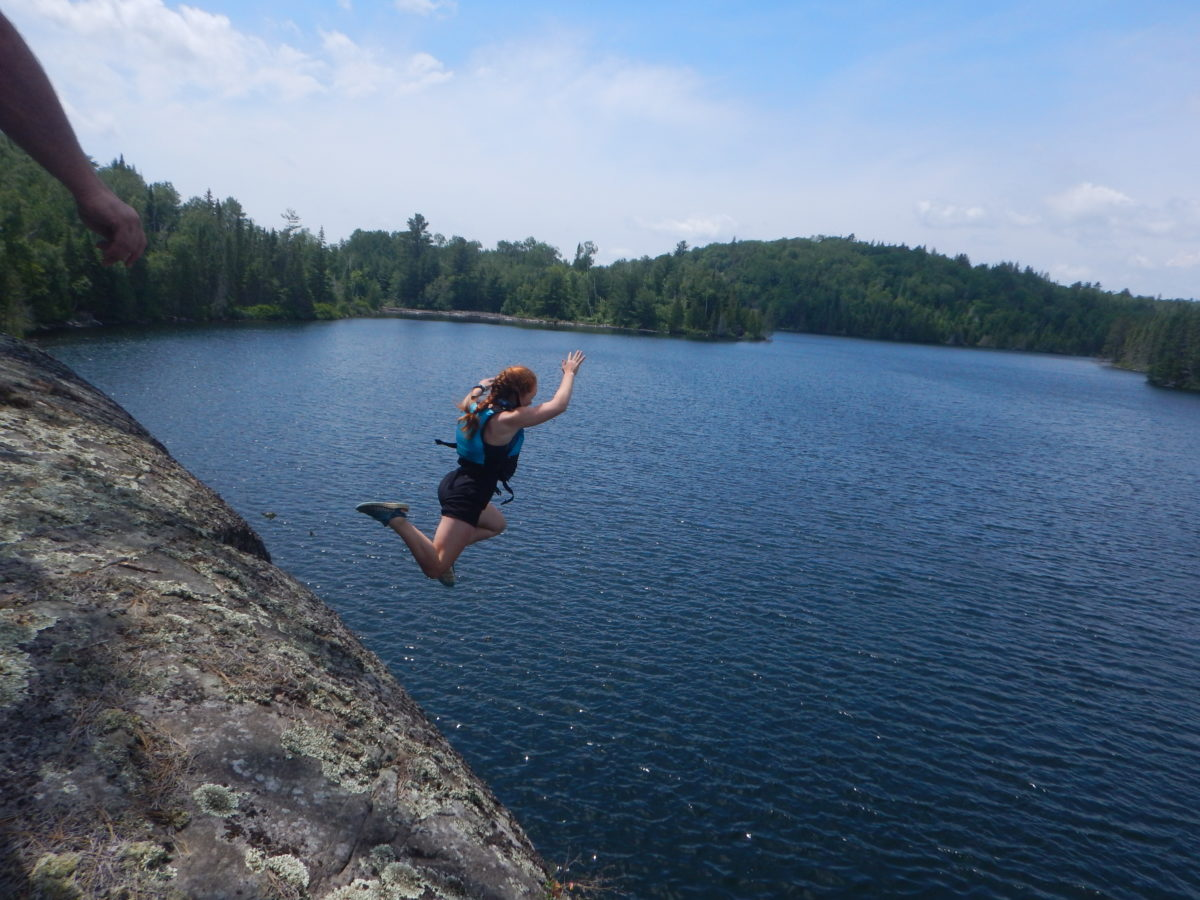
\includegraphics[width=0.62\textwidth]{./Chapter17/Figures/figure-bank-without-attention.jpg}};

\node [anchor=south,scale=1.2] (node1) at ([xshift=-2.5em,yshift=4.5em]y.north) {{$x$:源语言文本数据}};
\node [anchor=north,scale=1.2] (node2) at ([xshift=0.57em]node1.south){{$y$:目标语言文本数据}};

\draw[->,thick](x)to(encoder);
\draw[->,thick](encoder)to(decoder_left)node[right,xshift=-0.1cm,yshift=-1.25cm,scale=1.2]{{翻译}};
\draw[->,thick](decoder_left)to(y_hat);
\draw[->,thick](y)to(decoder_left);
\draw[->,thick](encoder)to(decoder_right)node[left,xshift=-3.1em,yshift=0.25cm,scale=1.2]{{生成图片}};
\draw[->,thick](decoder_right)to(figure);
\end{tikzpicture}
\caption{翻译+图片生成联合学习模型}
\label{fig:17-14}
\end{figure}
%----------------------------------------------------------------------------------------------------

%----------------------------------------------------------------------------------------
%    NEW SUB-SECTION
%----------------------------------------------------------------------------------------

\subsection{图像到文本的翻译}

\parinterval 图像到文本的转换也可以看作是广义上的翻译,简单来说,就是把图像作为唯一的输入,而输出是文本。其中,图像描述生成是最典型的图像到文本的翻译任务\upcite{DBLP:conf/ijcai/BernardiCEEEIKM17}。虽然,这部分内容并不是本书的重点,不过为了保证多模态翻译内容的完整性,这里对相关技术进行简要介绍。图像描述有时也被称看图说话、图像字幕生成,它在图像检索、智能导盲、人机交互等领域有着广泛的应用场景。

%----------------------------------------------------------------------------------------------------
\begin{figure}[htp]
\centering
\definecolor{color_gray}{rgb}{0.278,0.337,0.426}
\definecolor{color_green}{rgb}{0.663,0.82,0.557}
\definecolor{color_orange}{rgb}{0.957,0.694,0.514}
\definecolor{color_blue}{rgb}{0.335,0.708,0.735}
\tikzstyle{description} = [rectangle,rounded corners=1mm, minimum width=3cm,minimum height=0.6cm,text centered,draw,thick]
\begin{tikzpicture}[node distance = 0,scale = 0.8]
\tikzstyle{every node}=[scale=0.8]



\node(figure-1)[draw=white,scale=0.25] at (0,0){
\includegraphics[width=0.62\textwidth]{./Chapter17/Figures/figure-dog-with-hat.png}};
\node(ground-1)[rectangle,rounded corners, minimum width=5cm, minimum height=3.5cm,right of = figure-1, xshift=5cm,fill=gray!10,draw,thick,drop shadow]{};
\node(text-1)[right of = figure-1, xshift=3.6cm,yshift=2.1cm,scale=1.2]{{描述候选池}};
\node(text_1-1)[description, right of = figure-1, xshift=4.2cm,yshift=1.2cm,fill=gray!20]{{天空中有很多鸟。}};
\node(text_2-1)[description, right of = figure-1, xshift=5.3cm,yshift=0.5cm,fill=green!20]{{孩子从河岸上跳下来。}};
\node(text_3-1)[description, right of = figure-1, xshift=4.5cm,yshift=-0.2cm,fill=orange!20]{{狗在吐舌头。}};
\node(surd-1)[right of = text_3-1, xshift=2cm,scale=1.5]{\textcolor{red}{$\surd$}};
\node(text_4-1)[description, right of = figure-1, xshift=5.2cm,yshift=-0.9cm,fill=blue!20]{{男人戴着眼镜。}};
\node(point-1)[right of = figure-1, xshift=5cm,yshift=-1.4cm,scale=1.5]{...};
\draw[->,thick](figure-1)to([xshift=-0.1cm]ground-1.west);

\node(figure)[draw=white,scale=0.25]at ([xshift=20.0em]figure-1.east){
\includegraphics[width=0.62\textwidth]{./Chapter17/Figures/figure-dog-with-hat.png}};
\node(ground)[rectangle,rounded corners, minimum width=5cm, minimum height=1.5cm,right of = figure, xshift=5cm,yshift=-2.6em,fill=gray!10,draw,thick,drop shadow]{\large{图片中有\underline{\textcolor{red}{狗}},\underline{\textcolor{red}{帽子}},\underline{\quad\ }。}};
\node(dog)[rectangle,rounded corners, minimum width=1cm, minimum height=0.7cm,right of = figure, xshift=3cm,yshift=1.5cm,thick, draw,fill=orange!20,thick]{狗};
\node(hat)[rectangle,rounded corners, minimum width=1.5cm, minimum height=0.7cm,right of = figure, xshift=4.5cm,yshift=1.5cm,thick, draw,fill=green!20,thick]{帽子};
\draw[->, thick](figure.east)to([xshift=-0.1cm]dog.west)node[left,xshift=-0.2cm,yshift=-0.1cm,color=black]{图片检测};
\draw[->, thick]([yshift=-0.1cm]hat.south)to([yshift=0.1cm]ground.north)node[right,xshift=-0.2cm,yshift=0.5cm,color=black]{模板填充};

\node [anchor=north](pos1)at ([xshift=-3.8em,yshift=-1em]ground-1.south){(a) 基于检索的图像描述生成};
\node [anchor=north](pos2)at ([xshift=-3.8em,yshift=-1em]ground.south){(b) 基于模板的图像描述生成};

\end{tikzpicture}
\caption{图像描述传统方法}
\label{fig:17-15}
\end{figure}
%----------------------------------------------------------------------------------------------------

\parinterval 传统图像描述生成有两种范式:基于检索的方法和基于模板的方法。其中图\ref{fig:17-15}(a)展示了一个基于检索的图像描述生成实例,这种方法在图像描述的候选中选择一个描述输出。但是,弊端是所选择的句子可能会和图像很大程度上不相符。而\ref{fig:17-15}(b)展示的是一种基于模版的方法,这种方法需要在图像上提取视觉特征,然后把内容填在实现设计好的模板当中,这种方法的缺点是生成的图像描述过于呆板,“像是在一个模子中刻出来的”说的就是这个意思。近几年来 ,受到机器翻译领域等任务的启发,图像描述生成任务也开始大量使用编码器-解码器框架。这里会从基础的图像描述范式编码器-解码器框架展开\upcite{DBLP:conf/cvpr/VinyalsTBE15,DBLP:conf/icml/XuBKCCSZB15},并从编码器的改进和解码器的改进两个方面进行介绍。

%----------------------------------------------------------------------------------------
%    NEW SUBSUB-SECTION
%----------------------------------------------------------------------------------------

\subsubsection{1. 基础框架}

\parinterval 在编码器-解码器框架中,编码器将输入的图像转换为一种新的“表示”形式,这种“表示”包含了输入图像的所有信息。之后解码器把这种“表示”转换为自然语言描述。比如,可以通过卷积神经网络提取图像特征为一个向量表示。然后,利用长短时记忆网络(LSTMs)解码生成文字描述,这个过程中与机器翻译的解码过程类似。这种建模方式存在与\ref{sec:image-augmented-translation}描述一样的问题:生成的描述单词不一定需要所有的图像信息,将全局的图像信息送入模型中,可能会引入噪音。这时可以使用注意力机制来缓解该问题\upcite{DBLP:conf/icml/XuBKCCSZB15}。

%----------------------------------------------------------------------------------------
%    NEW SUBSUB-SECTION
%----------------------------------------------------------------------------------------

\subsubsection{2. 编码器的改进}

\parinterval 要想使编码器-解码器框架在图像描述生成中充分发挥作用,编码器也要更好的表示图像信息。对于编码器的改进,通常体现在向编码器中添加图像的语义信息\upcite{DBLP:conf/cvpr/YouJWFL16,DBLP:conf/cvpr/ChenZXNSLC17,DBLP:journals/pami/FuJCSZ17}和位置信息\upcite{DBLP:conf/cvpr/ChenZXNSLC17,DBLP:conf/ijcai/LiuSWWY17}。

\parinterval 图像的语义信息一般是指图像中存在的实体、属性、场景等等。如图\ref{fig:17-17}所示,从图像中利用属性或实体检测器提取出“jump”、“girl”、“river”、“bank”等属性词和实体词,将他们作为图像的语义信息编码的一部分,再利用注意力机制计算目标语言单词与这些属性词或实体词之间的注意力权重\upcite{DBLP:conf/cvpr/YouJWFL16}。当然,除了图像中的实体和属性作为语义信息外,也可以将图片的场景信息加入到编码器当中\upcite{DBLP:journals/pami/FuJCSZ17}。有关如何做属性、实体和场景的检测,涉及到目标检测任务的工作,例如Faster-RCNN\upcite{DBLP:journals/pami/RenHG017}、YOLO\upcite{DBLP:journals/corr/abs-1804-02767,DBLP:journals/corr/abs-2004-10934}等等,这里不再赘述。

%----------------------------------------------------------------------------------------------------
\begin{figure}[htp]
\centering
\tikzstyle{word} = [rectangle,thick,minimum width=2cm,minimum height=0.7cm,text centered,]
\begin{tikzpicture}[node distance = 0,scale = 0.9]
\tikzstyle{every node}=[scale=0.9]
\node(figure)[draw=white,scale=0.4] {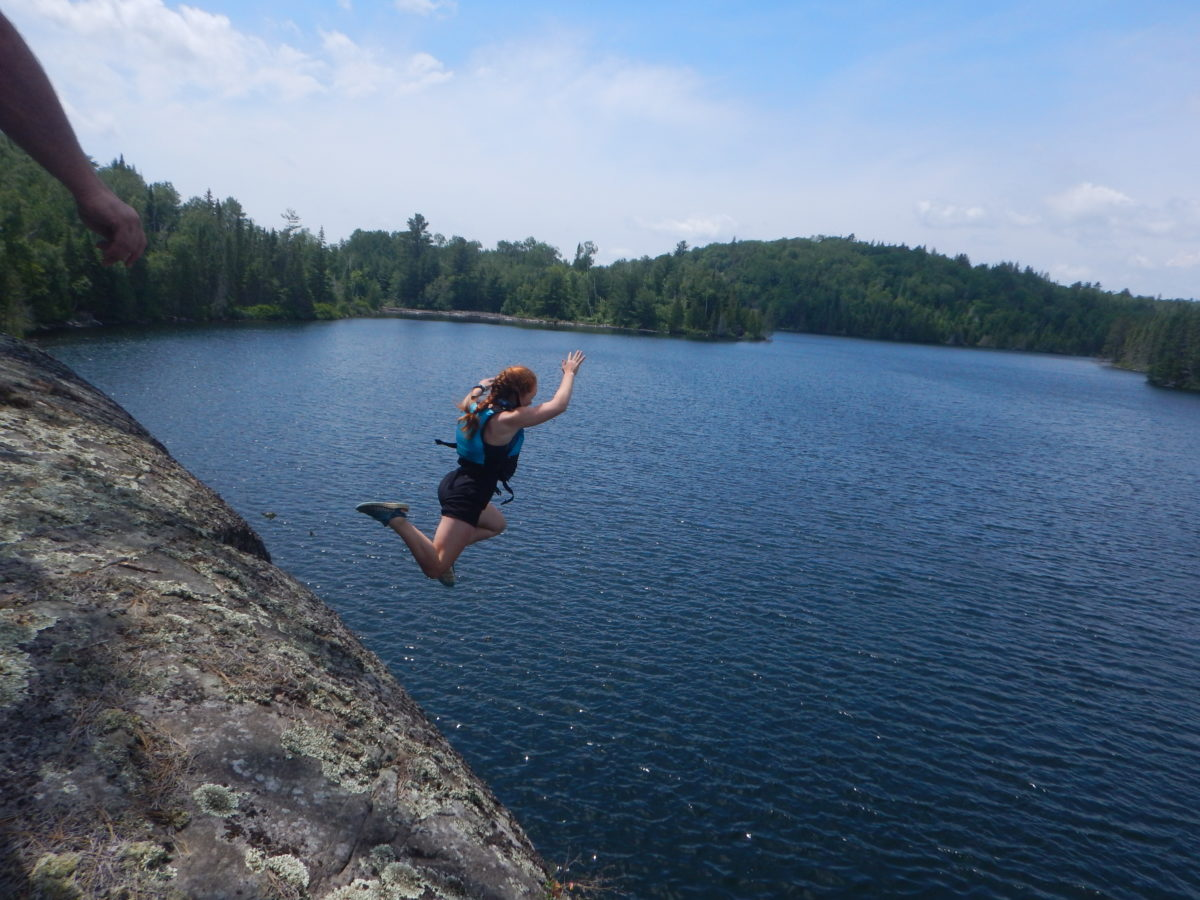
\includegraphics[width=0.62\textwidth]{./Chapter17/Figures/figure-bank-without-attention.jpg}};
\node(river)[word, right of = figure, xshift=5cm, yshift=0.35cm, fill=blue!45]{river};
\node(mountain)[word, above of = river, yshift=0.75cm, fill=blue!45]{mountain};
\node(child)[word, above of = mountain, yshift=0.75cm, fill=blue!15]{child};
\node(woman)[word, above of = child, yshift=0.75cm, fill=blue!25]{girl};
\node(jump)[word, below of = river, yshift=-0.75cm, fill=blue!30]{jump};
\node(bank)[word, below of = jump, yshift=-0.75cm, fill=blue!65]{bank};
\node(sky)[word, below of = bank, yshift=-0.75cm, fill=blue!30]{sky};
\node(tree)[word, below of = sky, yshift=-0.75cm, fill=blue!15]{tree};
\node(cir)[circle,thick, minimum width=0.6cm, xshift=8cm,  draw=black]{};
\node(decoder)[rectangle, rounded corners, minimum height=2.2em,minimum width=4.3em, right of = cir,xshift=3cm, draw=black, fill=blue!25]{\large{解码器}};
\node(yn_1)[below of = decoder,yshift=-2cm,scale=1.2]{$y_{<j}$};
\node(yn_2)[above of = decoder,yshift=2cm,scale=1.2]{$y_{j}$(bank)};

\draw[->, thick]([xshift=0.1cm]figure.east)to([xshift=2cm]figure.east);
\draw[-,thick]([xshift=-0.03cm]cir.east)to([xshift=0.03cm]cir.west);
\draw[-,thick]([yshift=0.03cm]cir.south)to([yshift=-0.03cm]cir.north);
\draw[->, thick]([xshift=0.1cm]cir.east)to([xshift=-0.1cm]decoder.west);
\draw[->, thick](yn_1)to([yshift=-0.1cm]decoder.south);
\draw[->, thick]([yshift=0.1cm]decoder.north)to(yn_2);

\draw[->, thick, color=blue!25]([xshift=0.05cm]woman.east)to([xshift=-0.05cm]cir.north);
\draw[->, thick, color=blue!15]([xshift=0.05cm]child.east)to([yshift=0.7em,xshift=0.4em]cir.west);
\draw[->, thick, color=blue!45]([xshift=0.05cm]mountain.east)to([yshift=0.5em,xshift=0.15em]cir.west);
\draw[->, thick, color=blue!45]([xshift=0.05cm]river.east)to([yshift=0.15em]cir.west);
\draw[->, thick, color=blue!30]([xshift=0.05cm]jump.east)to([yshift=-0.15em]cir.west);
\draw[->, very thick, color=blue!65]([xshift=0.05cm]bank.east)to([yshift=-0.5em,xshift=0.15em]cir.west);
\draw[->, thick, color=blue!30]([xshift=0.05cm]sky.east)to([yshift=-0.7em,xshift=0.4em]cir.west);
\draw[->, thick, color=blue!15]([xshift=0.05cm]tree.east)to([xshift=-0.05em]cir.south);
\end{tikzpicture}
\caption{编码器“显式”融入语义信息}
\label{fig:17-17}
\end{figure}
%----------------------------------------------------------------------------------------------------

\parinterval 以上的方法大都是将图像中的实体、属性、场景等映射到文字上,并把这些信息显式地输入到编码器中。另一种方式,把图像中的语义特征隐式地引入编码中\upcite{DBLP:conf/cvpr/ChenZXNSLC17}。例如,图像数据可以分解为三个通道(红、绿、蓝),简单来说,就是将图像的每一个像素点按照红色、绿色、蓝色分成三个部分,这样就将图像分成了三个通道。在很多图像中,不同通道伴随的特征是不一样的,可以将其作用于编码器。另一种方法是基于位置信息的编码增强。位置信息指的是图像中对象(物体)的位置。利用目标检测技术检测系统获得图中的对象和对应的特征,这样就确定了图中的对象位置。显然,这些信息可以加强编码器的表示能力\upcite{DBLP:conf/eccv/YaoPLM18}。

%----------------------------------------------------------------------------------------
%    NEW SUBSUB-SECTION
%----------------------------------------------------------------------------------------

\subsubsection{3. 解码器的改进}

\parinterval 由于解码器输出的是语言文字序列,因此需要考虑语言的特点对其进行改进。 例如,解码过程中, “the”,“on”,“at”这种介词或者冠词与图像的相关性较低\upcite{DBLP:conf/cvpr/LuXPS17}。因此,可以通过门控单元,控制视觉信号作用于文字生成的程度。另外,在解码过程中,生成的每个单词对应着图像的区域可能是不同的。因此也可以设计更为有效的注意力机制来捕捉解码器端对不同图像局部信息的关注程度\upcite{DBLP:conf/cvpr/00010BT0GZ18}。

\parinterval 除了更好地使生成文本与图像特征进行相互作用以外,还有一些改进方法。例如,用卷积神经网络或者Transformer代替解码器所使用的循环神经网络\upcite{DBLP:conf/cvpr/AnejaDS18}。或者使用更深层的神经网络学习动词或者形容词等视觉中不易表现出来的单词\upcite{DBLP:journals/mta/FangWCT18},其思想与深层神经机器翻译模型有相通之处(见{\chapterfifteen})。

%----------------------------------------------------------------------------------------
%    NEW SUB-SECTION
%----------------------------------------------------------------------------------------

\subsection{图像、文本到图像的翻译}

\parinterval 当生成的目标对象是图像时,问题就变为了图像生成任务。虽然,这个领域本身并不属于机器翻译,但是其使用的基本方法与机器翻译有类似之处。二者也可以相互借鉴。

\parinterval 在计算机视觉中,图像风格变换、图像超分辨率重建等任务,都可以被视为{\small\bfnew{图像到图像的翻译}}\index{图像到图像的翻译}(Image-to-Image Translation)\index{Image-to-Image Translation}问题。与机器翻译类似,这些问题的共同目标是学习从一个对象到另一个对象的映射,只不过这里的对象是指图像,而非机器翻译中的文字。例如,给定物体的轮廓生成真实物体图片,或者给定白天照片生成夜晚的照片等。图像到图像的翻译有广阔的应用场景,如图片补全、风格迁移等。{\small\bfnew{文本到图像的翻译}}\index{文本到图像的翻译}(Text-to-Image Translation)\index{Text-to-Image Translation}是指给定描述物体颜色和形状等细节的自然语言文字,生成对应的图像。该任务也可以看作是图像描述生成的逆任务。

\parinterval 无论是图像到图像的生成,还是文本到图像的生成,均可直接使用编码器-解码器框架进行实现。比如,在文本到图像生成中,可以使用机器翻译中的编码器对输入文本进行编码,之后用对抗生成网络将编码结果转化为图像\upcite{DBLP:conf/icml/ReedAYLSL16}。近些年,图像生成类任务也取得了很大的进展,这主要得益于生成对抗网络的使用\upcite{DBLP:conf/nips/GoodfellowPMXWOCB14,DBLP:journals/corr/abs-1908-06616,DBLP:journals/corr/DashGALA17}。在{\chapterthirteen}已经介绍了生成对抗网络,而且图像生成也不是本书的重点,感兴趣的读者可以参考{\chapterthirteen}的内容或者自行查阅相关文献进行了解。

%----------------------------------------------------------------------------------------
%    NEW SECTION
%----------------------------------------------------------------------------------------
\sectionnewpage
\section{篇章级翻译}

\parinterval 目前大多数机器翻译系统是句子级的。由于缺少了对篇章上下文信息的建模,在需要依赖上下文的翻译场景中,模型的翻译效果总是不尽人意。篇章级翻译的目的就是对篇章上下文信息进行建模,进而改善机器翻译在整个篇章上的翻译质量。篇章级翻译的概念在很早就已经出现\upcite{DBLP:journals/ac/Bar-Hillel60},随着近几年神经机器翻译取得了巨大进展,篇章级神经机器翻译也成为了重要的方向\upcite{DBLP:journals/corr/abs-1912-08494,DBLP:journals/corr/abs-1901-09115}。基于此,本节将对篇章级神经机器翻译的若干问题展开讨论。

%----------------------------------------------------------------------------------------
%    NEW SUB-SECTION
%----------------------------------------------------------------------------------------

\subsection{篇章级翻译的挑战}

\parinterval “篇章”在这里是指一系列连续的段落或句子所构成的整体,其中各个句子间从形式和内容上都具有一定的连贯性和一致性\upcite{jurafsky2000speech}。这些联系主要体现在衔接以及连贯两个方面。其中衔接体现在显性的语言成分和结构上,包括篇章中句子间的语法和词汇的联系,而连贯体现在各个句子之间的逻辑和语义的联系上。因此,篇章级翻译就是要将这些上下文之间的联系考虑在内,从而生成比句子级翻译更连贯和准确的翻译结果。实例\ref{eg:17-1}就展示了一个使用篇章信息进行机器翻译的实例。

\begin{example}
上下文句子:我/上周/针对/这个/问题/做出/解释/并/咨询/了/他的/意见/。

\hspace{2em} 待翻译句子:他/也/同意/我的/看法/。

\hspace{2em} 句子级翻译结果:He also agrees with me .

\hspace{2em} 篇章级翻译结果:{\red{And}} he {\red{agreed}} with me .

\label{eg:17-1}
\end{example}

\parinterval  不过由于不同语言的特性多种多样,上下文信息在篇章级翻译中的作用也不尽相同。比如,在德语中名词是分词性的,因此在代词翻译的过程中需要根据其先行词的词性进行区分,而这种现象在其它不区分名词词性的语言中是不存在的。这意味着篇章级翻译在不同的语种中可能对应不同的上下文现象。

\parinterval 正是这种上下文现象的多样性,使评价篇章级翻译模型的性能变得相对困难。目前篇章级机器翻译主要针对一些常见的上下文现象进行优化,比如代词翻译、省略、连接和词汇衔接等,而{\chapterfour}介绍的BLEU等通用自动评价指标通常对这些上下文依赖现象不敏感,因此篇章级翻译需要采用一些专用方法来对这些具体现象进行评价。

\parinterval 在统计机器翻译时代就已经有大量的研究工作专注于篇章信息的建模,这些工作大多针对某一具体的上下文现象,比如,篇章结构\upcite{DBLP:conf/anlp/MarcuCW00,foster2010translating,DBLP:conf/eacl/LouisW14}、代词回指\upcite{DBLP:conf/iwslt/HardmeierF10,DBLP:conf/wmt/NagardK10,DBLP:conf/eamt/LuongP16,}、词汇衔接\upcite{tiedemann2010context,DBLP:conf/emnlp/GongZZ11,DBLP:conf/ijcai/XiongBZLL13,xiao2011document}和篇章连接词\upcite{DBLP:conf/sigdial/MeyerPZC11,DBLP:conf/hytra/MeyerP12,}等。区别于篇章级统计机器翻译,篇章级神经机器翻译不需要针对某一具体的上下文现象构造相应的特征,而是通过翻译模型本身从上下文句子中抽取和融合的上下文信息。通常情况下,篇章级机器翻译可以采用局部建模的手段将前一句或者周围几句作为上下文送入模型。针对需要长距离上下文的情况,也可以使用全局建模的手段直接从篇章的所有句子中提取上下文信息。近几年多数研究工作都在探索更有效的局部建模或全局建模方法,主要包括改进输入\upcite{DBLP:conf/discomt/TiedemannS17,DBLP:conf/naacl/BawdenSBH18,DBLP:conf/wmt/GonzalesMS17,DBLP:journals/corr/abs-1910-07481}、多编码器结构\upcite{DBLP:journals/corr/JeanLFC17,DBLP:journals/corr/abs-1805-10163,DBLP:conf/emnlp/ZhangLSZXZL18}、层次结构\upcite{DBLP:conf/naacl/MarufMH19,DBLP:conf/acl/HaffariM18,DBLP:conf/emnlp/YangZMGFZ19,DBLP:conf/ijcai/ZhengYHCB20}以及基于缓存的方法\upcite{DBLP:conf/coling/KuangXLZ18,DBLP:journals/tacl/TuLSZ18}等。

\parinterval 此外,篇章级机器翻译面临的另外一个挑战是数据稀缺。篇章级机器翻译所需要的双语数据需要保留篇章边界,数量相比于句子级双语数据要少很多。除了在之前提到的端到端方法中采用预训练或者参数共享的手段(见{\chaptersixteen}),也可以采用新的建模手段来缓解数据稀缺问题。这类方法通常将篇章级翻译流程进行分离:先训练一个句子级的翻译模型,再通过一些额外的模块来引入上下文信息。比如,在句子级翻译模型的推断过程中,通过在目标端结合篇章级语言模型引入上下文信息\upcite{DBLP:conf/discomt/GarciaCE19,DBLP:journals/tacl/YuSSLKBD20,DBLP:journals/corr/abs-2010-12827},或者基于句子级的翻译结果,使用两阶段解码等手段引入上下文信息,进而对句子级翻译结果进行修正\upcite{DBLP:conf/aaai/XiongH0W19,DBLP:conf/acl/VoitaST19,DBLP:conf/emnlp/VoitaST19}。

%----------------------------------------------------------------------------------------
%    NEW SUBSUB-SECTION
%----------------------------------------------------------------------------------------

\subsection{篇章级翻译的评价}\label{sec:17-3-2}

\parinterval BLEU等自动评价指标能够在一定程度上反映译文的整体质量,但是并不能有效地评估篇章级翻译模型的性能。这是由于很多标准测试集中需要篇章上下文的情况比例相对较少。而且,$n$-gram的匹配很难检测到一些具体的语言现象,这使得研究人员很难通过BLEU得分来判断篇章级翻译模型的效果。

\parinterval 为此,研究人员总结了机器翻译任务中存在的上下文现象,并基于此设计了相应的自动评价指标。比如针对篇章中代词的翻译问题,首先借助词对齐工具确定源语言中的代词在译文和参考答案中的对应位置,然后通过计算译文中代词的准确率和召回率等指标对代词翻译质量进行评价\upcite{DBLP:conf/iwslt/HardmeierF10,DBLP:conf/discomt/WerlenP17}。针对篇章中的词汇衔接,使用{\small\sffamily\bfseries{词汇链}}\index{词汇链}(Lexical Chain\index{Lexical Chain})\footnote{词汇链指篇章中语义相关的词所构成的序列。}等来获取能够反映词汇衔接质量的分数,然后通过加权的方式与常规的BLEU或METEOR等指标结合在一起\upcite{DBLP:conf/emnlp/WongK12,DBLP:conf/discomt/GongZZ15}。针对篇章中的连接词,使用候选词典和词对齐工具对源文中连接词的正确翻译结果进行计数,计算其准确率\upcite{DBLP:conf/cicling/HajlaouiP13}。

\parinterval 除了直接对译文打分,也有一些工作针对特有的上下文现象手工构造了相应的测试套件用于评价翻译质量。测试套件中每一个测试样例都包含一个正确翻译的结果,以及多个错误结果,一个理想的翻译模型应该对正确的翻译结果评价最高,排名在所有错误结果之上,此时就可以根据模型是否能挑选出正确翻译结果来评估其性能。这种方法可以很好地衡量翻译模型在某一特定上下文现象上的处理能力,比如词义消歧\upcite{DBLP:conf/wmt/RiosMS18}、代词翻译\upcite{DBLP:conf/naacl/BawdenSBH18,DBLP:conf/wmt/MullerRVS18}和一些衔接问题\upcite{DBLP:conf/acl/VoitaST19}等。但是该方法也存在使用范围受限于测试集的语种和规模的缺点,因此扩展性较差。

%----------------------------------------------------------------------------------------
%    NEW SUB-SECTION
%----------------------------------------------------------------------------------------

\subsection{篇章级翻译的建模}

\parinterval 在理想情况下,篇章级翻译应该以整个篇章为单位作为模型的输入和输出。然而由于现实中篇章对应的序列过长,因此直接建模整个篇章序列难度很大,这使得主流的序列到序列模型很难直接使用。一种思路是采用能够处理超长序列的模型对篇章序列建模,比如,使用{\chapterfifteen}中提到的处理长序列的Transformer模型就是一种的解决方法\upcite{Kitaev2020ReformerTE}。不过,这类模型并不针对篇章级翻译的具体问题,因此并不是篇章级翻译中的主流方法。

\parinterval 现在常见的端到端做法还是从句子级翻译出发,通过额外的模块来对篇章中的上下文句子进行表示,然后提取相应的上下文信息并融入到当前句子的翻译过程中。形式上,篇章级翻译的建模方式如下:
\begin{eqnarray}
\funp{P}(\seq{Y}|\seq{X})&=&\prod_{i=1}^{T}{\funp{P}(Y_i|X_i,D_i)}
\label{eq:17-3-1}
\end{eqnarray}
其中,$\seq{X}$和$\seq{Y}$分别为源语言篇章和目标语言篇章,$X_i$和$Y_i$分别为源语言篇章和目标语言篇章中的第$i$个句子,$T$表示篇章中句子的数目。为了简化问题,这里假设源语言和目标语言具有相同的句子数目$T$,而且两个篇章间句子是顺序对应的。$D_i$表示翻译第$i$个句子时所对应的上下文句子集合,理想情况下,$D_i$中包含源语言篇章和目标语言篇章中所有除第$i$句之外的句子,但实践中通常仅使用其中的部分句子作为上下文。

\parinterval 上下文范围的选取是篇章级神经机器翻译需要着重考虑的问题,比如上下文句子的多少\upcite{agrawal2018contextual,Werlen2018DocumentLevelNM,DBLP:conf/naacl/MarufMH19},是否考虑目标端上下文句子\upcite{DBLP:conf/discomt/TiedemannS17,agrawal2018contextual}等。此外,不同的上下文范围也对应着不同的建模方法,接下来将对一些典型的方法进行介绍,包括改进输入\upcite{DBLP:conf/discomt/TiedemannS17,DBLP:conf/naacl/BawdenSBH18,DBLP:conf/wmt/GonzalesMS17,DBLP:journals/corr/abs-1910-07481}、多编码器模型\upcite{DBLP:journals/corr/JeanLFC17,DBLP:journals/corr/abs-1805-10163,DBLP:conf/emnlp/ZhangLSZXZL18}、层次结构模型\upcite{DBLP:conf/emnlp/WangTWL17,DBLP:conf/emnlp/TanZXZ19,Werlen2018DocumentLevelNM}以及基于缓存的方法\upcite{DBLP:conf/coling/KuangXLZ18,DBLP:journals/tacl/TuLSZ18}。

%----------------------------------------------------------------------------------------
%    NEW SUBSUB-SECTION
%----------------------------------------------------------------------------------------

\subsubsection{1. 输入形式}

\parinterval 一种简单的方法是直接复用传统的序列到序列模型,将篇章中待翻译句子与其上下文句子拼接后作为模型输入。如实例\ref{eg:17-3-1}所示,这种做法不需要改动模型结构,操作简单,适用于大多数神经机器翻译系统\upcite{DBLP:conf/discomt/TiedemannS17,agrawal2018contextual,DBLP:conf/discomt/ScherrerTL19}。但是由于过长的序列会导致模型难以训练,通常只会选取局部的上下文句子进行拼接,比如只拼接源语言端前一句或者周围几句\upcite{DBLP:conf/discomt/TiedemannS17}。此外,也可以引入目标语言端的上下文\upcite{DBLP:conf/naacl/BawdenSBH18,agrawal2018contextual,DBLP:conf/discomt/ScherrerTL19},在解码时拼接目标语言端上下文和当前句同样会带来一定的性能提升。但是过大的窗口会造成推断速度的下降\upcite{agrawal2018contextual},因此通常只考虑前一个目标语言句子。

\begin{example}
传统模型训练输入:

\hspace{10em}源语言:你/看到/了/吗/?

\hspace{10em}目标语言:Do you see them ?

\vspace{0.5em}
\qquad\ 改进后模型训练输入:

\hspace{10em}源语言:{\red{他们/在/哪/?\ <sep>\ }}\ 你/看到/了/吗/?

\hspace{10em}目标语言:Do you see them ?

\label{eg:17-3-1}
\end{example}

\parinterval 其他改进输入的做法相比于拼接的方法要复杂一些,首先需要对篇章进行处理,得到词汇链\footnote{词汇链指篇章中语义相关的词所构成的序列。}或者篇章嵌入等信息\upcite{DBLP:conf/wmt/GonzalesMS17,DBLP:journals/corr/abs-1910-07481},然后将这些信息与当前句子一起送入模型中。目前,这种预先提取篇章信息的方法是否适合机器翻译还有待论证。

%----------------------------------------------------------------------------------------
%    NEW SUBSUB-SECTION
%----------------------------------------------------------------------------------------

\subsubsection{2. 多编码器结构}


\parinterval 另一种思路是对传统的编码器-解码器框架进行更改,引入额外的编码器来对上下文句子进行编码,该结构被称为多编码器结构\upcite{DBLP:conf/acl/LiLWJXZLL20,DBLP:conf/discomt/SugiyamaY19}。这种结构最早被应用在基于循环神经网络的篇章级翻译模型中\upcite{DBLP:journals/corr/JeanLFC17,DBLP:conf/coling/KuangX18,DBLP:conf/naacl/BawdenSBH18,DBLP:conf/pacling/YamagishiK19},后期证明在Transformer模型上同样适用\upcite{DBLP:journals/corr/abs-1805-10163,DBLP:conf/emnlp/ZhangLSZXZL18}。图\ref{fig:17-18}展示了一个基于Transformer模型的多编码器结构,基于源语言当前待翻译句子的编码表示$\mathbi{h}$和上下文句子的编码表示$\mathbi{h}^{\textrm {pre}}$,模型首先通过注意力机制提取句子间上下文信息$\mathbi{d}$:
\begin{eqnarray}
\mathbi{d}&=&\textrm{Attention}(\mathbi{h},\mathbi{h}^{\textrm {pre}},\mathbi{h}^{\textrm {pre}})
\label{eq:17-3-3}
\end{eqnarray}
其中,$\mathbi{h}$作为Query(查询),$\mathbi{h}^{\textrm pre}$作为Key(键)和Value(值)。然后通过门控机制将待翻译句子中每个位置的编码表示和该位置对应的上下文信息进行融合,具体方式如下:
\begin{eqnarray}
\lambda_{t}&=&\sigma(\mathbi{W}_{\lambda}[\mathbi{h}_{t};\mathbi{d}_{t}]+\mathbi{b}_{\lambda})
\label{eq:17-3-5}\\
\widetilde{\mathbi{h}_{t}}&=&\lambda_{t}\mathbi{h}_{t}+(1-\lambda_{t})\mathbi{d}_{t}
\label{eq:17-3-4}
\end{eqnarray}
其中,$\widetilde{\mathbi{h}}$为融合了上下文信息的最终序列表示结果,$\widetilde{\mathbi{h}_{t}}$为其第$t$个位置的表示。$\mathbi{W}_{\lambda}$和$\mathbi{b}_{\lambda}$为模型可学习的参数,$\sigma$为Sigmoid函数,用来获取门控权值$\lambda$。除了在编码端融合源语言上下文信息,也可以直接用类似机制在解码器内完成源语言上下文信息的融合\upcite{DBLP:conf/emnlp/ZhangLSZXZL18}。

%----------------------------------------------
\begin{figure}[htp]
    \centering
	\definecolor{color1}{rgb}{1,0.725,0.058}
\tikzstyle{coder} = [rectangle,thick,rounded corners,minimum width=2.8cm,minimum height=1.1cm,text centered,draw=black!,fill=blue!30,drop shadow]
\tikzstyle{attention} = [rectangle,thick,rounded corners,minimum width=2.6cm,minimum height=0.9cm,text centered,draw=black,fill=green!30!white,drop shadow]

\begin{tikzpicture}[node distance = 0,scale = 0.7]
\tikzstyle{every node}=[scale=0.7]
\node(encoder_c)[coder]{\large{编码器}};
\node(encoder_s)[coder, right of = encoder_c, xshift=3.5cm, fill=red!30]{\large{编码器}};
\node(h_pre)[above of = encoder_c, yshift=1.3cm,scale=1.3]{${\mathbi{h}}^{\rm pre}$};
\node(h)[above of = encoder_s, yshift=1.3cm,scale=1.3]{$\mathbi{h}$};
\node(cir)[circle,very thick, right of = h, draw=black!90,minimum width=0.5cm,xshift=1.1cm]{};
\draw[-,very thick,draw=black!90]([xshift=0.04cm]cir.west)--([xshift=-0.04cm]cir.east);
\draw[-,very thick,draw=black!90]([yshift=-0.04cm]cir.north)--([yshift=0.04cm]cir.south);
\node(last)[below of = encoder_c, yshift=-1.3cm]{\large{前一个句子}};
\node(current)[below of = encoder_s, yshift=-1.3cm]{\large{当前句子}};
\node(attention_left)[attention, above of = encoder_c, xshift=2.4cm,yshift=3.1cm]{\large{注意力机制}};
\node(d)[above of = attention_left, yshift=1.1cm,scale=1.3]{$\mathbi{d}$};
\node(ground)[rectangle, thick, rounded corners, minimum width=5cm, minimum height=5.5cm, right of = encoder_s, xshift=4.4cm,yshift=2.2cm, draw=black, fill=gray!10]{};
\node(decoder)[above of = encoder_s, xshift=3.1cm]{\large{解码器}};
\node(attention_right)[attention, right of = attention_left, xshift=5.4cm,yshift=-0.4cm]{\large{注意力机制}};
\node(target)[right of = current, xshift=5.3cm]{\large{目标语言句子(位置$j$之前)}};
\node(point_below)[right of = encoder_s, xshift=5.3cm]{\Huge{...}};
\node(point_above)[above of = attention_right, yshift=1.8cm]{\Huge{...}};
\node(target_above)[above of = attention_right, yshift=3.3cm]{\large{目标语言句子}};

\draw[->,thick](last)to([yshift=-0.05cm]encoder_c.south);
\draw[->,thick](current)to([yshift=-0.05cm]encoder_s.south);
\draw[->,thick](target.north)to([yshift=-0.05cm]point_below.south);
\draw[->,thick]([yshift=0.05cm]encoder_c.north)to([yshift=0.03cm]h_pre.south);
\draw[->,thick]([yshift=0.05cm]encoder_s.north)to(h.south);
\draw[->,thick]([yshift=0cm]h.north)to([yshift=0.95cm]h.north);
\draw[->,thick,in=270,out=90]([yshift=-0.15cm]h_pre.north)to([xshift=1.25cm,yshift=0.9cm]h_pre.north);
\draw[->,thick,in=270,out=80]([yshift=-0.15cm]h_pre.north)to([xshift=2.4cm,yshift=0.9cm]h_pre.north);
\draw[->,thick]([yshift=0.03cm]attention_left.north)to([yshift=0.1cm]d.south);
\draw[->,thick]([xshift=-0.03cm]h.east)to([xshift=-0.03cm]cir.west);
\draw[->,thick](point_below.north)to([yshift=2.03cm]point_below.north);
\draw[->,thick](attention_right.north)to([yshift=-0.03cm]point_above.south);
\draw[->,thick](point_above.north)to([yshift=0.83cm]point_above.north);
\draw[->,thick, in=270,out=0]([xshift=0.2cm]cir.east)to([xshift=3cm,yshift=0.88cm]cir.east);
\draw[->,thick, in=270,out=0]([xshift=0.2cm]cir.east)to([xshift=2cm,yshift=0.88cm]cir.east);
\draw[->,very thick,]([xshift=0.1cm]d.east)to([xshift=1.92cm]d.east)to([yshift=0.03cm]cir.north);
\end{tikzpicture}
    \caption{多编码器结构\upcite{DBLP:conf/acl/LiLWJXZLL20}}
    \label{fig:17-18}
\end{figure}
%----------------------------------------------

\parinterval 此外,由于多编码器结构引入了额外的模块,模型整体参数量大大增加,同时增加了模型训练的难度。为此,一些研究人员提出使用句子级模型预训练的方式来初始化模型参数\upcite{DBLP:journals/corr/JeanLFC17,DBLP:conf/emnlp/ZhangLSZXZL18},或者将两个编码器的参数进行共享来降低模型复杂度\upcite{DBLP:conf/pacling/YamagishiK19,DBLP:conf/coling/KuangX18,DBLP:journals/corr/abs-1805-10163}。

%----------------------------------------------------------------------------------------
%    NEW SUBSUB-SECTION
%----------------------------------------------------------------------------------------

\subsubsection{3. 层次结构模型}


\parinterval 多编码器结构通过额外的编码器对前一句进行编码,但是当处理更多上下文句子的时候仍然面临效率低下的问题。为了捕捉更大范围的上下文,可以采用层次结构来对更多的上下文句子进行建模。层次结构是一种有效的序列表示方法,而且人类语言中天然就具有层次性,比如,句法树、篇章结构树等。类似的思想也成功的应用在基于树的句子级翻译模型中(见{\chaptereight}和{\chapterfifteen})。

\parinterval 图\ref{fig:17-19}描述了一个基于层次注意力的模型结构\upcite{Werlen2018DocumentLevelNM}。首先通过翻译模型的编码器获取前$K$个句子的词序列编码表示$(\mathbi{h}^{\textrm{pre}1},\dots,\mathbi{h}^{\textrm{pre}K})$,然后针对前文每个句子的词序列编码表示$\mathbi{h}^{\textrm{pre}k}$,使用词级注意力提取当前句子内部的注意力信息$\mathbi{s}^{k}$,然后在这$K$个句子级上下文信息$\mathbi{s}=(\mathbi{s}^1,\dots,\mathbi{s}^K)$的基础上,使用句子级注意力提取篇章上下文信息$\mathbi{d}$。由于上下文信息$\mathbi{d}$的获取涉及到词级和句子级两个不同层次的注意力操作,因此将该过程称为层次注意力。实际上,这种方法并没有使用语言学的篇章层次结构。但是,句子级注意力在归纳统计意义上的篇章结构,因此这种方法也可以捕捉不同句子之间的关系。

%----------------------------------------------
\begin{figure}[htp]
    \centering
	
\begin{tikzpicture}[node distance = 0,scale = 0.8]
\tikzstyle{every node}=[scale=0.8]

\foreach \x in {1,2,3,4}
	\node[draw,inner sep=0pt,minimum height=1em,minimum width=1.6em,fill=red!35,rounded corners=1pt] (c1_\x) at (0em+2em*\x, 0em){};
\node[anchor=north] (hpre) at ([yshift=1.8em]c1_1.north) {${\mathbi{h}}^ {\textrm{pre}k}$};
\foreach \x in {1,2,3}
	\node[draw,inner sep=0pt,minimum height=1em,minimum width=1.6em,fill=red!35,rounded corners=1pt] (c2_\x) at (11em+2em*\x, 0em){};
\node[anchor=north] (hpre) at ([yshift=1.8em]c2_1.north) {${\mathbi{h}}^ {\textrm{pre}1}$};
\foreach \x in {1,2,3,4,5}
	\node[draw,inner sep=0pt,minimum height=1em,minimum width=1.6em,fill=red!35,rounded corners=1pt] (c3_\x) at (18.4em+2em*\x, 0em){};,minimum width=1em

\foreach \x in {1,2,3,4,5}
	\node[draw,inner sep=0pt,minimum height=1em,minimum width=1.6em,fill=blue!35,rounded corners=1pt] (c4_\x) at (18.4em+2em*\x, 10.4em){};

%\node[inner sep=0pt,minimum size=1em,fill=ugreen,circle,thick] (c5) at (9em, 7em){};
\node[draw,inner sep=0pt,minimum size=1.2em,fill=green!30!white,circle,thick] (qs) at (18.6em, 6.4em){};
\node[draw,inner sep=0pt,minimum size=1.2em,fill=green!30!white,circle,thick] (qw) at (18.6em, 4.4em){};
\node[anchor=north] (qslab) at ([xshift=-0.8em,yshift=1em]qs.north) {${\mathbi{q}}_s$};
\node[anchor=north] (qwlab) at ([xshift=-0.8em,yshift=1em]qw.north) {${\mathbi{q}}_w$};

\node[draw,thick,inner sep=0pt, minimum size=1.2em, circle,thick] (sigma) at (24.4em, 8em){};
\draw[-,thick] (sigma.0) -- (sigma.180);
\draw[-,thick] (sigma.90) -- (sigma.-90);

\node[draw,fill=orange!35,inner sep=0pt, minimum size=1.2em, circle,thick] (add1) at (5em, 3em){};
\node[draw,fill=orange!35,inner sep=0pt, minimum size=1.2em, circle,thick] (add2) at (15em, 3em){};
\node[draw,fill=orange!35,inner sep=0pt, minimum size=1.2em, circle,thick] (add3) at (10em, 5.2em){};
\node[anchor=north] (cond) at ([xshift=-1.2em,yshift=0.5em]add3.north) {${\mathbi{d}_t}$};
\node[anchor=north] (cons1) at ([xshift=-1em,yshift=0.5em]add2.north) {${\mathbi{s}}^1$};
\node[anchor=north] (consj) at ([xshift=-1em,yshift=0.5em]add1.north) {${\mathbi{s}}^k$};
\begin{pgfonlayer}{background}
\node[draw,rounded corners=2pt,drop shadow,fill=white, minimum width=8.3em,thick][fit=(c1_1)(c1_4)](box1){};
\node[draw,rounded corners=2pt,drop shadow,fill=white,minimum width=6.4em,thick][fit=(c2_1)(c2_3)](box2){};
\node[draw,rounded corners=2pt,drop shadow,fill=white,minimum width=10.5em,thick][fit=(c3_1)(c3_5)](box3){};
\node[draw,rounded corners=2pt,drop shadow,fill=white,minimum width=10.3em,thick][fit=(c4_1)(c4_5)](box4){};
%\node[draw,rounded corners=2pt,inner xsep=6pt,drop shadow,fill=white][fit=(c5)](box5){};
\end{pgfonlayer}

\node[draw=violet,densely dotted,minimum width=1.9em, minimum height=2.1em,very thick] (n1) at (24.4em,0em){};
\node[draw=violet,densely dotted,minimum width=1.8em, minimum height=2em,very thick] (n2) at (24.4em,10.4em){};
%\node[] at (24.4em, -1.5em){$\mathbi{x}_\mathbi{t}$};
\node[text=ublue] at (10.5em, 0em) {\small\bfnew{...}};
\node[text=ublue] (hh) at (-0.8em, 0em) {\small\bfnew{...}};

\draw[->,thick, out=70, in=-120] ([yshift=0.1em]c1_1.90) to ([yshift=-0.1em]add1.-120);
%node[xshift=-0.4em,yshift=1.2em]{$ \mathbi{h}^ {\textrm j}$}
\draw[->,thick, out=80, in=-100] ([yshift=0.1em]c1_2.90) to ([yshift=-0.1em]add1.-100);
\draw[->,thick, out=100, in=-80] ([yshift=0.1em]c1_3.90) to ([yshift=-0.1em]add1.-80);
\draw[->,thick, out=110, in=-60] ([yshift=0.1em]c1_4.90) to ([yshift=-0.1em]add1.-60);

\draw[->,thick, out=70, in=-110] ([yshift=0.1em]c2_1.90) to ([yshift=-0.1em]add2.-110);
\draw[->,thick, out=90, in=-90] ([yshift=0.1em]c2_2.90) to ([yshift=-0.1em]add2.-90);
\draw[->,thick, out=110, in=-70] ([yshift=0.1em]c2_3.90) to ([yshift=-0.1em]add2.-70);


\draw[->,thick, out=30, in=-130] ([yshift=0.1em]add1.90) to ([yshift=-0.1em]add3.-120);
\draw[->,thick, out=150, in=-50] ([yshift=0.1em]add2.90) to ([yshift=-0.1em]add3.-70);
\draw[->,thick, ugreen!60,out=160,in=-10] ([xshift=-0.1em]qs.160) to ([xshift=0.1em]add3.0);
\draw[->,thick, ugreen!60,out=180,in=0] ([xshift=-0.1em]qw.180) to ([xshift=0.1em]add2.0);
\draw[->,thick, ugreen!60,out=170,in=-10] ([xshift=-0.1em]qw.160) to ([xshift=0.1em]add1.0);

\draw[->,thick] ([yshift=0.1em]n1.135) .. controls ([xshift=-2em]n1.130) and ([xshift=2em]qw.0) .. ([xshift=0.1em]qw.0);
\draw[->,thick] ([yshift=0.1em]n1.120) .. controls ([xshift=-2em,yshift=1em]n1.120) and ([xshift=3em]qs.0) .. ([xshift=0.1em]qs.0);
\draw[->,thick] ([yshift=0.1em]n1.90) node[yshift=0.5em,right]{$ {\mathbi{h}}_t$}-- ([yshift=-0.1em]sigma.-90);
\draw[->,thick] ([yshift=0.1em]sigma.90) -- ([yshift=-0.1em]n2.-90);
\draw[->,thick] ([yshift=0.1em]n2.90) -- node[right]{$ \widetilde{\mathbi{h}}_t$}([yshift=2em]n2.90);

\draw[decorate,decoration={brace, mirror},gray, thick] ([yshift=-2em]hh.-180) -- node[font=\footnotesize,text=black,below]{前几个句子}([yshift=-2em]box2.0);
\draw[decorate,decoration={brace, mirror},gray, thick] ([yshift=-2em]box3.-180) -- node[font=\footnotesize,text=black,below]{当前句子}([yshift=-2em]box3.0);
\draw[->, thick, rounded corners=2pt] ([yshift=0.1em]add3.90) -- ([yshift=2.1em]add3.90) -- ([xshift=-0.1em]sigma.180);


%annotation
%\node[fill=red!30,rounded corners=1pt,inner sep=0pt,minimum size=1em] (a1) at (2em,-4.5em) {};
%\node[anchor=west,font=\footnotesize] (w1) at ([xshift=0.4em]a1.east) {编码表示};

%\node[anchor=west,fill=orange!30,rounded corners=1pt,inner sep=0pt,minimum size=1em] (a2) at ([xshift=2em]w1.east) {};
%\node[anchor=west,font=\footnotesize] (w2)at ([xshift=0.4em]a2.east) {层次注意力};

%\node[anchor=west,fill=blue!30,rounded corners=1pt,inner sep=0pt,minimum size=1em] (a3) at ([xshift=2em]w2.east) {};
%\node[anchor=west,font=\footnotesize] at ([xshift=0.4em]a3.east) {融合上下文信息的编码表示};
\end{tikzpicture}





    \caption{层次注意力结构\upcite{Werlen2018DocumentLevelNM}}
    \label{fig:17-19}
\end{figure}
%----------------------------------------------

\parinterval 为了增强模型的表示能力,层次注意力中并未直接使用当前句子第$t$个位置的编码表示$\mathbi{h}_{t}$作为注意力操作的Query(查询),而是通过两个线性变换分别获取词级注意力和句子级注意力的查询$\mathbi{q}_{w}$ 和$\mathbi{q}_{s}$,定义如公式\eqref{eq:17-3-6}\eqref{eq:17-3-8},其中${\mathbi W}_w$、${\mathbi W}_s$、${\mathbi b}_w$、${\mathbi b}_s$分别是两个线性变换的权重和偏置。

\begin{eqnarray}
\mathbi{q}_{w}&=&{\mathbi W}_w \mathbi{h}_t+{\mathbi b}_w
\label{eq:17-3-6}\\
\mathbi{q}_{s}&=&{\mathbi W}_s \mathbi{h}_t+{\mathbi b}_s
\label{eq:17-3-8}
\end{eqnarray}


\noindent 之后,分别计算词级和句子级注意力模型。需要注意的是句子级注意力添加了一个前馈全连接网络子层FFN。其具体计算方式如下:

\begin{eqnarray}
\mathbi{s}^k&=&\textrm{WordAttention}(\mathbi{q}_{w},\mathbi{h}^{\textrm {pre}k},\mathbi{h}^{\textrm{pre}k})
\label{eq:17-3-7}\\
\mathbi{d}_t&=&\textrm{FFN}(\textrm{SentAttention}(\mathbi{q}_{s},\mathbi{s},\mathbi{s}))
\label{eq:17-3-9}
\end{eqnarray}

\noindent 其中,$\textrm{WordAttention}(\cdot)$和$\textrm{SentAttention}(\cdot)$都是标准的自注意力模型。在得到最终的上下文信息$\mathbi{d}$后,模型同样采用门控机制(如公式\eqref{eq:17-3-4} 和公式\eqref{eq:17-3-5})与$\mathbi{h}$进行融合来得到一个上下文相关的当前句子表示$\widetilde{\mathbi{h}}$。

\parinterval 通过层次注意力,模型可以在词级和句子级两个维度从多个句子中提取更充分的上下文信息,除了用于编码器,也可以用于解码器来获取目标语言的上下文信息。基于层次注意力,为了进一步编码整个篇章的上下文信息,研究人员提出选择性注意力来对篇章中整体上下文进行有选择的信息提取\upcite{DBLP:conf/naacl/MarufMH19}。此外,也有研究人员使用循环神经网络\upcite{DBLP:conf/emnlp/WangTWL17}、 记忆网络\upcite{DBLP:conf/acl/HaffariM18}、胶囊网络\upcite{DBLP:conf/emnlp/YangZMGFZ19}和片段级相对注意力\upcite{DBLP:conf/ijcai/ZhengYHCB20}等结构来对多个上下文句子进行上下文信息提取。

%----------------------------------------------------------------------------------------
%    NEW SUBSUB-SECTION
%----------------------------------------------------------------------------------------

\subsubsection{4. 基于缓存的方法}

\parinterval 除了以上提到的建模方法,还有一类基于缓存的方法\upcite{DBLP:journals/tacl/TuLSZ18,DBLP:conf/coling/KuangXLZ18}。这类方法最大的特点在于将篇章翻译看作一个连续的过程,即依次翻译篇章中的每一个句子,该过程中通过一个额外的缓存来记录一些相关信息,且在每个句子的推断过程中都使用这个缓存来提供上下文信息。图\ref{fig:17-20}描述了一种基于缓存的篇章级翻译模型结构\upcite{DBLP:journals/tacl/TuLSZ18}。 在这里,翻译模型基于循环神经网络(见{\chapterten}),但是这种方法同样适用于包括Transformer在内的其他神经机器翻译模型。

\parinterval 模型中篇章上下文的建模依赖于缓存的读和写操作。缓存的写操作指的是:按照一定规则,将翻译历史中一些译文单词对应的上下文向量作为键,将其解码器端的隐藏状态作为值,共同写入到缓存中。而缓存的读操作是指将待翻译句子中第$t$个单词的上下文向量$\mathbi{C}_t$作为Query(查询),与缓存中的所有键分别进行匹配,并根据其匹配程度进行带权相加,最后得到当前待翻译句子的篇章上下文信息 $\mathbi{d}$。 该方法中,解码器端隐藏状态$\mathbi{s}_t$与对应位置的上下文信息$\mathbi{d}_t$的融合也是基于门控机制。事实上,由于该方法中缓存空间是有限的,其内容的更新也存在一定的规则:在当前句子的翻译结束后,如果单词$y_t$的对应信息未曾写入缓存,则写入其中的空槽或者替换最久未使用的键值对;如果$y_t$ 已作为翻译历史存在于缓存中,则将对应的键值对按照以下规则进行更新:
\begin{eqnarray}
\mathbi{k}_{i}&=&\frac{\mathbi{k}_{i}+\mathbi{c}_{t}}{2}
\label{eq:17-3-10}\\
\mathbi{v}_{i}&=&\frac{\mathbi{v}_{i}+\mathbi{s}_{t}}{2}
\label{eq:17-3-11}
\end{eqnarray}
其中,$i$表示$y_t$在缓存中的位置,$\mathbi{k}_{i}$和$\mathbi{v}_{i}$分别为缓存中对应的键和值。这种方法缓存的都是目标语言历史的词级表示,因此能够解决一些词汇衔接的问题,比如词汇一致性和一些搭配问题,产生更连贯的翻译结果。
%----------------------------------------------
\begin{figure}[htp]
    \centering
	
\begin{tikzpicture}
%\tikzstyle{every node}=[scale=0.8]
	\tikzstyle{prob}=[minimum width=0.4em, fill=blue!20,inner sep=0pt]
\node[draw,fill=yellow!30,inner sep=0pt,minimum width=3em,minimum height=5em](key) at (0,0){};
\draw[] ([yshift=0.5em]key.180) -- ([yshift=0.5em]key.0);
\draw[] ([yshift=1.5em]key.180) -- ([yshift=1.5em]key.0);
\draw[] ([yshift=-0.5em]key.180) -- ([yshift=-0.5em]key.0);
\draw[] ([yshift=-1.5em]key.180) -- ([yshift=-1.5em]key.0);
\node[draw,fill=green!30!white,inner sep=0pt,minimum width=3em,minimum height=5em](value) at (3em,0){};
\draw[] ([yshift=0.5em]value.180) -- ([yshift=0.5em]value.0);
\draw[] ([yshift=1.5em]value.180) -- ([yshift=1.5em]value.0);
\draw[] ([yshift=-0.5em]value.180) -- ([yshift=-0.5em]value.0);
\draw[] ([yshift=-1.5em]value.180) -- ([yshift=-1.5em]value.0);

\node[anchor=south,font=\footnotesize,inner sep=0pt] at ([yshift=0.1em]key.north){键};
\node[anchor=south,font=\footnotesize,inner sep=0pt] at ([yshift=0.1em]value.north){值};
\node[anchor=south,font=\footnotesize,inner sep=0pt] (cache)at ([yshift=2em,xshift=1.5em]key.north){\small\bfnew{缓存}};

\node[draw,anchor=east,thick,minimum size=1.8em,fill=orange!30] (dt) at ([yshift=2.1em,xshift=-4em]key.west){${\mathbi{d}}_{t}$};
\node[anchor=north,font=\footnotesize] (readlab) at ([xshift=2.8em,yshift=0.3em]dt.north){\red{读取}};
\node[draw,anchor=east,thick,minimum size=1.8em,fill=green!30!white] (st) at ([xshift=-3.7em]dt.west){${\mathbi{s}}_{t}$};
\node[draw,anchor=east,thick,minimum size=1.8em,fill=red!30] (st2) at ([xshift=-0.85em,yshift=3.5em]dt.west){$ \widetilde{\mathbi{s}}_{t}$};

%\node[draw,anchor=north,circle,inner sep=0pt, minimum size=1.2em,fill=yellow] (add) at ([yshift=-1em]st2.south){+};
\node[draw,thick,inner sep=0pt, minimum size=1.1em, circle] (add) at ([yshift=-1.5em]st2.south){};
\draw[-,thick] (add.0) -- (add.180);
\draw[-,thick] (add.90) -- (add.-90);

\node[anchor=north,inner sep=0pt,font=\footnotesize,text=red] at ([xshift=-0em,yshift=-0.5em]add.south){融合};

\node[draw,anchor=east,thick,minimum size=1.8em,fill=yellow!30] (ct) at ([xshift=-2em,yshift=-3.5em]st.west){$ {\mathbi{C}}_{t}$};
\node[anchor=north,font=\footnotesize] (matchlab) at ([xshift=6.7em,yshift=-0.1em]ct.north){\red{匹配}};

\node[anchor=east] (y) at ([xshift=-6em,yshift=1em]st.west){$\mathbi{y}_{t-1}$};

\node[draw,anchor=east,minimum width=7em,minimum height=1.4em,fill=blue!30] (output) at ([xshift=-2.6em,yshift=2.6em]st2.west){};

\node[anchor=south] (yt) at ([yshift=4.2em]output.north){$\mathbi{y}_{t}$};
\draw[] ([xshift=-0.7em]output.90) -- ([xshift=-0.7em]output.-90);
\draw[] ([xshift=-2.1em]output.90) -- ([xshift=-2.1em]output.-90);
\draw[] ([xshift=0.7em]output.90) -- ([xshift=0.7em]output.-90);
\draw[] ([xshift=2.1em]output.90) -- ([xshift=2.1em]output.-90);

\foreach \x/\y in {1/2,2/1,3/5,4/1,5/1,6/1,7/3,8/4,9/2,10/3,11/5,12/10,13/2,14/5,15/5,16/5,17/5}
	\node[draw=blue!25,anchor=south,prob,minimum height=0.2em*\y] at ([yshift=1em,xshift=-3.65em+0.4em*\x]output.north){};
	
\begin{pgfonlayer}{background}
\node[inner sep=3pt,draw,dotted,rounded corners=2pt,very thick][fit=(key)(value)(cache)](box){};
\end{pgfonlayer}

\draw[-latex,dashed,very thick,out=-145,in=10] ([yshift=1em]box.180) to (dt.0);
%node[above,font=\footnotesize,text=red,rotate=25]{reading}
\draw[-latex,dashed,very thick,out=-5,in=-170] (ct.0) to ([yshift=-2.5em]box.180);
%node[above,font=\footnotesize,text=red,pos=0.7,rotate=8]{matching}
\draw[-,thick,out=0,in=-135](st.0) to (add.-135);
\draw[-,thick,out=180,in=-45](dt.180) to (add.-45);
\draw[-latex,thick] (add.90) -- (st2.-90);
\draw[-latex,thick,out=100,in=-100] (ct.90) to (output.-90);
\draw[-latex,thick,out=180,in=-100] (st2.180) to (output.-90);
\draw[-latex,thick,out=80,in=-100] (y.90) to (output.-90);
\draw[-latex,thick] (output.90) -- ([yshift=1em]output.90);
\draw[-latex,thick] ([yshift=-1.2em]yt.-90) -- (yt.-90);
\end{tikzpicture}
    \caption{基于缓存的解码器结构\upcite{DBLP:journals/tacl/TuLSZ18}}
    \label{fig:17-20}
\end{figure}
%----------------------------------------------

%----------------------------------------------------------------------------------------
%    NEW SUB-SECTION
%----------------------------------------------------------------------------------------

\subsection{在推断阶段结合篇章上下文}

\parinterval 前面介绍的方法主要是对篇章中待翻译句子的上下文句子进行建模,通过端到端的方式对上下文信息进行提取和融合。由于篇章级双语数据相对稀缺,这种复杂的篇章级翻译模型很难得到充分训练,通常可以采用两阶段训练或参数共享的方式来缓解这个问题。此外,由于句子级双语数据更为丰富,一个自然的想法是以高质量的句子级翻译模型为基础,通过在推断过程中结合上下文信息来构造篇章级翻译模型。

\parinterval 在句子级翻译模型中引入目标语言端的篇章级语言模型是一种结合上下文信息的常用手段\upcite{DBLP:conf/discomt/GarciaCE19,DBLP:journals/tacl/YuSSLKBD20,DBLP:journals/corr/abs-2010-12827}。 相比于篇章级双语数据,篇章级单语数据更容易获取。在双语数据稀缺的情况下,通过引入目标语言端的篇章级语言模型可以更充分的利用这些单语数据,比如,可以把这个语言模型与翻译模型做插值,也可以将其作为重排序阶段的一种特征。
%----------------------------------------------
\begin{figure}[htp]
    \centering
	\tikzstyle{encoder} = [rectangle,thick,rounded corners,minimum width=4.3em,minimum height=2.2em,text centered,draw=black,fill=red!30]
\tikzstyle{decoder} = [rectangle,thick,rounded corners,minimum width=4.3em,minimum height=2.2em,text centered,draw=black,fill=blue!25]
\tikzstyle{attention} = [rectangle,thick,rounded corners,minimum width=2.6cm,minimum height=2.2em,text centered,draw=black,fill=green!25]

\begin{tikzpicture}[node distance = 0,scale = 0.75]
\tikzstyle{every node}=[scale=0.75]
\node(decoder_left)[decoder]{\normalsize{解码器}};
\node(decoder_right)[decoder, right of = decoder_left, xshift=2.2cm]{\normalsize{解码器}};
\node(encoder_left)[encoder, above of = decoder_left, yshift=1.6cm]{\normalsize{编码器}};
\node(encoder_right)[encoder, above of = decoder_right, yshift=1.6cm]{\normalsize{编码器}};
\node(text_left)[below of = encoder_left, yshift=1.5cm]{\normalsize{前文}};
\node(text_right)[below of = encoder_right, yshift=1.5cm]{\normalsize{源语言句子}};
\node(text_top)[above of = decoder_right, yshift=-1.6cm]{\normalsize{句子级翻译结果}};
\node(title_1)[above of = text_left, xshift=1.1cm, yshift=3cm]{\large\bfnew{一阶段翻译}};
\node(ground2)[rectangle,very thick,rounded corners,minimum width=5cm,minimum height=5.8cm,right of = decoder_right,xshift=5.3cm,yshift=1.6cm,draw=black,dashed]{};
\node(ground1)[rectangle,thick,rounded corners,minimum width=3.3cm,minimum height=5cm,right of = decoder_right,xshift=4.8cm,yshift=1.58cm,draw=black,fill=yellow!15]{};
\node(attention_below)[attention, right of = decoder_right, xshift=4.8cm]{\normalsize{注意力机制}};
\node(attention_above)[attention, above of = attention_below, yshift=1.6cm]{\normalsize{注意力机制}};
\node(ffn)[attention, above of = attention_above, yshift=1.6cm, fill=blue!8]{\normalsize{前馈神经网络}};
\node [right of = attention_above, xshift=2.35cm,yshift=2.5cm,scale=1.2]{\footnotesize{解码器}};
\node(n)[right of = attention_above, xshift=2.4cm,scale=1.5]{$\times N$};
\node(text_2)[above of = ffn, yshift=1.9cm]{\normalsize{基于上下文的修正结果}};
\node(title_2)[right of = title_1, xshift=6.3cm]{\large\bfnew{二阶段翻译}};
%\node(text_rright)[right of = text_right, xshift=5.5cm]{\normalsize{句子级翻译结果}};

\draw[->,very thick]([yshift=-0.1cm]text_left.south)to(encoder_left.north);
\draw[->,very thick]([yshift=-0.1cm]text_right.south)to(encoder_right.north);
\draw[->,very thick](encoder_left.south)to(decoder_left.north);
\draw[->,very thick](encoder_right.south)to(decoder_right.north);
\draw[->,very thick](decoder_right.south)to([yshift=0.1cm]text_top.north);
%\draw[->,very thick]([yshift=0.2cm]text_rright.north)to(attention_below.south);
\draw[->,very thick](attention_below.north)to(attention_above.south);
\draw[->,very thick](attention_above.north)to([yshift=-0.05cm]ffn.south);
\draw[->,very thick](ffn.north)to([yshift=-0.05cm]text_2.south);
\draw[->,very thick]([yshift=-0.05em]text_top.south) -- ([yshift=-4.8em]decoder_right.south) -- ([yshift=-4.78em]attention_below.south) --(attention_below.south);
\draw[-,very thick,dashed]([xshift=1.25cm,yshift=-3cm]decoder_right.east)to([xshift=1.25cm,yshift=6.5cm]decoder_right.east);
\draw[->,very thick,draw=gray,rounded corners=2pt] (encoder_left.south)--([yshift=-0.3cm]encoder_left.south)--([yshift=-0.3cm,xshift=3.42cm]encoder_left.south)--([xshift=-2.25cm]attention_above.west)--(attention_above.west);
\draw[->,very thick,draw=gray,rounded corners=2pt] (encoder_right.south)--([yshift=-0.3cm]encoder_right.south)--([yshift=-0.3cm,xshift=3.42cm]encoder_left.south)--([xshift=-2.25cm]attention_above.west)--(attention_above.west);
\draw[->,very thick,draw=gray,rounded corners=2pt](decoder_left.south)--([yshift=-0.3cm]decoder_left.south)--([yshift=-0.3cm,xshift=3.42cm]decoder_left.south)--([xshift=-2.25cm]attention_below.west)--(attention_below.west);
\draw[->,very thick,draw=gray,rounded corners=2pt](decoder_right.south)--([yshift=-0.3cm]decoder_right.south)--([yshift=-0.3cm,xshift=3.42cm]decoder_left.south)--([xshift=-2.25cm]attention_below.west)--(attention_below.west);
\end{tikzpicture}
    \caption{两阶段翻译}
    \label{fig:17-21}
\end{figure}
%----------------------------------------------

\parinterval 另一种方法是两阶段翻译。这种方法不影响句子级翻译模型的推断过程,而是在完成翻译后使用额外的模块进行第二阶段的翻译\upcite{DBLP:conf/aaai/XiongH0W19,DBLP:conf/acl/VoitaST19}。如图\ref{fig:17-21}所示,这种两阶段翻译的做法相当于将篇章级翻译的问题进行了分离和简化:在第一阶段翻译中使用句子级翻译模型完成对篇章中某个句子的翻译,为了进一步地引入篇章上下文信息,第二阶段的翻译过程在第一阶段翻译结果的基础上,利用两次注意力操作,融合并引入源语言和目标语言的篇章上下文信息和当前句子信息。该方法适用于篇章级双语数据稀缺的场景。基于类似的思想,也可以使用后编辑的做法对翻译结果进行修正。区别于两阶段翻译的方法,后编辑的方法无需参考源语言信息,只利用目标语言端的上下文信息对译文结果进行修正\upcite{DBLP:conf/emnlp/VoitaST19}。

%----------------------------------------------------------------------------------------
%    NEW SECTION
%----------------------------------------------------------------------------------------
\sectionnewpage
\section{小结及拓展阅读}

\parinterval 使用更大上下文进行机器翻译建模是极具潜力的研究方向,包括多模态翻译在内的多个领域也非常活跃。有许多问题值得进一步思考与讨论:

\begin{itemize}
\vspace{0.5em}
\item 本章仅对音频处理和语音识别进行了简单的介绍,具体内容可以参考一些经典书籍,比如关于信号处理的基础知识\upcite{Oppenheim2001DiscretetimeSP,Quatieri2001DiscreteTimeSS},以及语音识别的传统方法\upcite{DBLP:books/daglib/0071550,Huang2001SpokenLP}和基于深度学习的最新方法\upcite{benesty2008automatic}。
\vspace{0.5em}
\item 此外,语音翻译的一个重要应用是机器同声传译。机器同声传译的一个难点在于不同语言的文字顺序不同。目前,同声传译的一种思路是基于目前已经说出的语音进行翻译\upcite{DBLP:conf/acl/MaHXZLZZHLLWW19},比如,等待源语$k$个词语,然后再进行翻译,同时改进束搜索方式来预测未来的词序列,从而提升准确度\upcite{DBLP:conf/emnlp/ZhengMZH19}。或者,对当前语音进行翻译,但需要判断翻译的词是否能够作为最终结果,已决定是否根据之后的语音重新进行翻译\upcite{DBLP:conf/naacl/DalviDSV18,DBLP:journals/corr/ChoE16}。第二种思路是动态预测当前时刻是应该继续等待还是开始翻译,这种方式更符合人类进行同传的行为。但是这种策略的难点在于标注每一时刻的决策状态十分耗时且标准难以统一,目前主流的方式是利用强化学习方法\upcite{DBLP:conf/eacl/NeubigCGL17,DBLP:conf/emnlp/GrissomHBMD14},对句子进行不同决策方案采样,最终学到最优的决策方案。此外,还有一些工作设计不同的学习策略\upcite{DBLP:conf/acl/ZhengLZMLH20,DBLP:conf/emnlp/ZhengZMH19,DBLP:conf/acl/ZhengZMH19}或改进注意力机制\upcite{DBLP:conf/acl/ArivazhaganCMCY19}以提升机器同声传译的性能。
\vspace{0.5em}

\item 在多模态机器翻译任务和篇章级机器翻译任务中,数据规模往往受限,导致模型训练困难,很难取得较好的性能。比如在篇章级机器翻译中,一些研究工作对这类模型的上下文建模能力进行了探索\upcite{DBLP:conf/discomt/KimTN19,DBLP:conf/acl/LiLWJXZLL20},发现模型在小数据集上对上下文信息的利用并不能带来明显的性能提升。针对数据稀缺导致的训练问题,一些研究人员通过调整训练策略使得模型更容易捕获上下文信息\upcite{DBLP:journals/corr/abs-1903-04715,DBLP:conf/acl/SaundersSB20,DBLP:conf/mtsummit/StojanovskiF19}。除了训练策略的调整,也可以使用数据增强的方式(例如,构造伪数据)来提升整体数据量\upcite{DBLP:conf/emnlp/GokhaleBBY20,DBLP:conf/eccv/Tang0ZWY20,DBLP:conf/discomt/SugiyamaY19},或者使用预训练的手段来利用额外地单语或图像数据\upcite{DBLP:conf/aaai/ZhouPZHCG20,DBLP:conf/iclr/SuZCLLWD20,DBLP:journals/corr/abs-1911-03110}。
\vspace{0.5em}
\end{itemize}














